\documentclass{beamer}
\usepackage[italian]{babel}
\usetheme{Berkeley}
\usepackage{graphicx}
\usepackage{booktabs}
% Taken from Lena Herrmann at 
% http://lenaherrmann.net/2010/05/20/javascript-syntax-highlighting-in-the-latex-listings-package
\usepackage{listings,lstautogobble}
\usepackage{color} %use color
\definecolor{mygreen}{rgb}{0,0.6,0}
\definecolor{mygray}{rgb}{0.5,0.5,0.5}
\definecolor{mymauve}{rgb}{0.58,0,0.82}
% Copyright 2017 Sergei Tikhomirov, MIT License
% https://github.com/s-tikhomirov/solidity-latex-highlighting/

\usepackage{listings, xcolor}

\definecolor{verylightgray}{rgb}{.97,.97,.97}

\lstdefinelanguage{Solidity}{
	keywords=[1]{anonymous, assembly, assert, balance, break, call, callcode, case, catch, class, constant, continue, constructor, contract, debugger, default, delegatecall, delete, do, else, emit, event, experimental, export, external, false, finally, for, function, gas, if, implements, import, in, indexed, instanceof, interface, internal, is, length, library, log0, log1, log2, log3, log4, memory, modifier, new, payable, pragma, private, protected, public, pure, push, require, return, returns, revert, selfdestruct, send, solidity, storage, struct, suicide, super, switch, then, this, throw, transfer, true, try, typeof, using, value, view, while, with, addmod, ecrecover, keccak256, mulmod, ripemd160, sha256, sha3}, % generic keywords including crypto operations
	keywordstyle=[1]\color{blue}\bfseries,
	keywords=[2]{address, bool, byte, bytes, bytes1, bytes2, bytes3, bytes4, bytes5, bytes6, bytes7, bytes8, bytes9, bytes10, bytes11, bytes12, bytes13, bytes14, bytes15, bytes16, bytes17, bytes18, bytes19, bytes20, bytes21, bytes22, bytes23, bytes24, bytes25, bytes26, bytes27, bytes28, bytes29, bytes30, bytes31, bytes32, enum, int, int8, int16, int24, int32, int40, int48, int56, int64, int72, int80, int88, int96, int104, int112, int120, int128, int136, int144, int152, int160, int168, int176, int184, int192, int200, int208, int216, int224, int232, int240, int248, int256, mapping, string, uint, uint8, uint16, uint24, uint32, uint40, uint48, uint56, uint64, uint72, uint80, uint88, uint96, uint104, uint112, uint120, uint128, uint136, uint144, uint152, uint160, uint168, uint176, uint184, uint192, uint200, uint208, uint216, uint224, uint232, uint240, uint248, uint256, var, void, ether, finney, szabo, wei, days, hours, minutes, seconds, weeks, years},	% types; money and time units
	keywordstyle=[2]\color{teal}\bfseries,
	keywords=[3]{block, blockhash, coinbase, difficulty, gaslimit, number, timestamp, msg, data, gas, sender, sig, value, now, tx, gasprice, origin},	% environment variables
	keywordstyle=[3]\color{violet}\bfseries,
	identifierstyle=\color{black},
	sensitive=false,
	comment=[l]{//},
	morecomment=[s]{/*}{*/},
	commentstyle=\color{gray}\ttfamily,
	stringstyle=\color{red}\ttfamily,
	morestring=[b]',
	morestring=[b]"
}

\lstset{
	language=Solidity,
	backgroundcolor=\color{verylightgray},
	extendedchars=true,
	basicstyle=\footnotesize\ttfamily,
	showstringspaces=false,
	showspaces=false,
	numbers=left,
	numberstyle=\footnotesize,
	numbersep=9pt,
	tabsize=2,
	breaklines=true,
	showtabs=false,
	captionpos=b
}

%Customize a bit the look
\lstset{ %
autogobble = true,
backgroundcolor=\color{white}, % choose the background color; you must add \usepackage{color} or \usepackage{xcolor}
basicstyle=\footnotesize, % the size of the fonts that are used for the code
breakatwhitespace=false, % sets if automatic breaks should only happen at whitespace
breaklines=true, % sets automatic line breaking
captionpos=b, % sets the caption-position to bottom
commentstyle=\color{mygreen}, % comment style
deletekeywords={...}, % if you want to delete keywords from the given language
escapeinside={<@}{@>}, % if you want to add LaTeX within your code
escapechar={|},
extendedchars=true, % lets you use non-ASCII characters; for 8-bits encodings only, does not work with UTF-8
frame=single, % adds a frame around the code
keywordstyle=\color{blue}, % keyword style
% language=Octave, % the language of the code
morekeywords={*,...}, % if you want to add more keywords to the set
numbers=left, % where to put the line-numbers; possible values are (none, left, right)
numbersep=0pt, % how far the line-numbers are from the code
numberstyle=\tiny\color{mygray}, % the style that is used for the line-numbers
rulecolor=\color{black}, % if not set, the frame-color may be changed on line-breaks within not-black text (e.g. comments (green here))
showspaces=false, % show spaces everywhere adding particular underscores; it overrides 'showstringspaces'
showstringspaces=false, % underline spaces within strings only
showtabs=false, % show tabs within strings adding particular underscores
stepnumber=1, % the step between two line-numbers. If it's 1, each line will be numbered
stringstyle=\color{mymauve}, % string literal style
tabsize=2, % sets default tabsize to 2 spaces
title=\lstname, % show the filename of files included with \lstinputlisting; also try caption instead of title
}
%END of listing package%

\definecolor{darkgray}{rgb}{.4,.4,.4}
\definecolor{purple}{rgb}{0.65, 0.12, 0.82}

%define Javascript language
\lstdefinelanguage{JavaScript}{
keywords={typeof, new, true, false, catch, function, return, null, catch, switch, var, if, while, do, else, case, break, for, of, const, async, await},
keywordstyle=\color{blue}\bfseries,
ndkeywords={class, export, boolean, throw, implements, import},
ndkeywordstyle=\color{darkgray}\bfseries,
identifierstyle=\color{black},
sensitive=false,
comment=[l]{//},
morecomment=[s]{/*}{*/},
commentstyle=\color{purple}\ttfamily,
stringstyle=\color{red}\ttfamily,
morestring=[b]',
morestring=[b]"
}

\lstset{
language=JavaScript,
extendedchars=true,
basicstyle=\fontsize{8}{9}\selectfont\ttfamily,
showstringspaces=false,
showspaces=false,
numbers=left,
numberstyle=\fontsize{8}{9}\selectfont,
numbersep=0pt,
tabsize=2,
breaklines=true,
showtabs=false,
captionpos=b
}
\graphicspath{{figures/}}

\title{Condividere informazioni in modo \\
sicuro combinando Git e Blockchain}
\author{Laureando: Paolo Speziali \\ Relatore: Luca Grilli}
\institute{Università degli Studi di Perugia - Dipartimento di Ingegneria\\Corso di laurea triennale in Ingegneria Informatica ed Elettronica\\[\medskipamount]
      
\includegraphics[width=0.3\textwidth]{figures/logo_unipg.png}
 }
\logo{
\includegraphics[height=1cm]{favicon.png}}
\date{A.A. 2020/2021}

\begin{document}
\begin{frame}
	\titlepage % beamer's \maketitle
\end{frame}
\begin{frame}
	\frametitle{Indice}
	\tableofcontents
\end{frame}
\section{Il Problema}
\begin{frame}
	\frametitle{La digitalizzazione}
	È in atto, negli ultimi anni, un piano di \textbf{digitalizzazione} delle PA.
	Esso mira all'evoluzione tecnologica di tutte le sue mansioni e alla creazione
	di portali web per il cittadino.
	L'esigenza di questa trasformazione si è fatta sentire anche da parte
	dell'\textbf{Unione Europea}, che con il \textbf{Recovery Fund}
	ci sta fornendo i fondi per attuarla, ben \textbf{11,75 milioni di euro}.
	\begin{figure}
		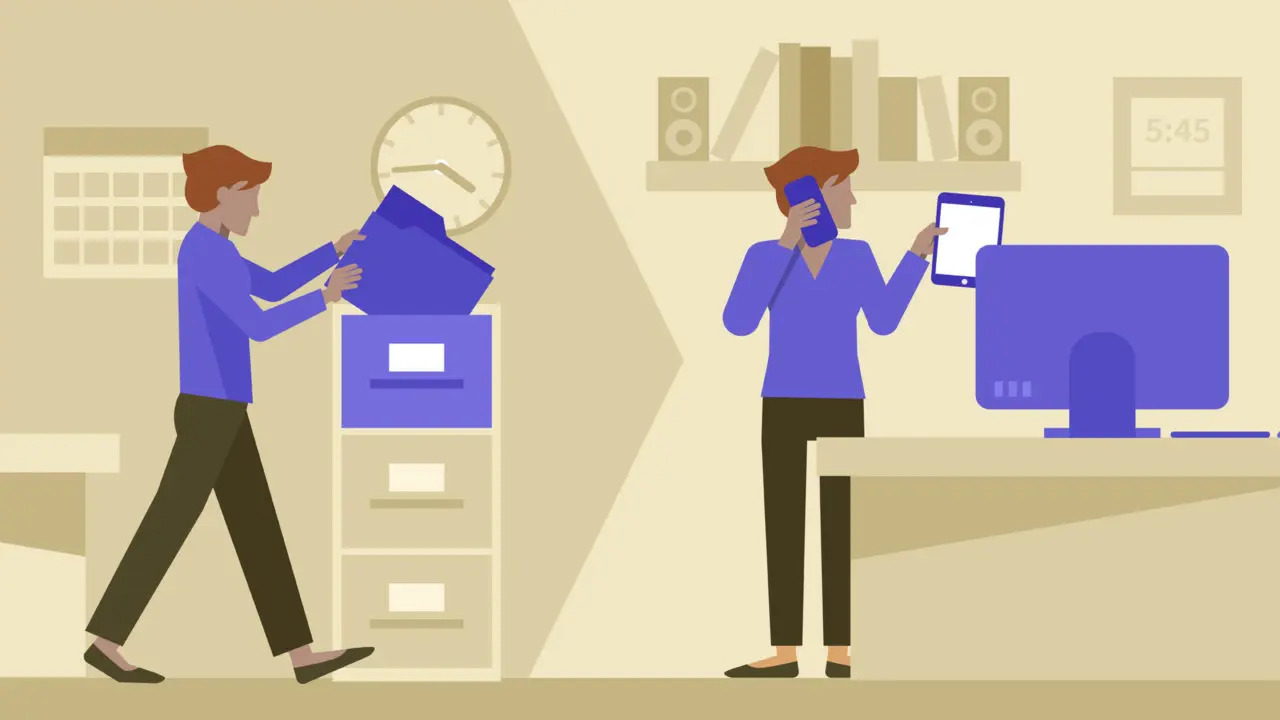
\includegraphics[width=0.55\textwidth]{digitalizzazione.jpg}
		% https://www.agendadigitale.eu/documenti/digitalizzazione-della-pa-in-italia-la-strategia-delle-tre-c/
	\end{figure}
\end{frame}

\begin{frame}
	\frametitle{Il problema della burocrazia}
	Il più grande avversario della digitalizzazione è la \textbf{burocrazia} italiana:
	i suoi processi sono \textbf{lenti} e \textbf{complessi} anche a causa dell'\textbf{importanza}
	dei documenti da gestire.
	È necessaria una \textbf{sburocratizzazione}
	grazie a degli strumenti digitali che permettano di \textbf{salvare},
	\textbf{validare} e \textbf{condividere} documenti senza abbassare il \textbf{livello di sicurezza}.
	\medskip
	\begin{figure}
		
\includegraphics[width=0.65\textwidth]{buro.jpg}
		% https://www.identitafutura.it/burocrazia-allitaliana/
	\end{figure}
\end{frame}

\begin{frame}
	\frametitle{Gli strumenti attuali}
	\medskip
	\begin{columns}
		\column{0.65\textwidth}
		Uno strumento digitale solitamente segue uno di questi due paradigmi:
		\textbf{centralizzato} e \textbf{distribuito}. \\
		Nel primo un'entità centrale si occupa dell'\textbf{immagazzinamento} e della \textbf{verifica} dei dati
		degli utenti.\\ Ciò ha diversi \textbf{svantaggi}:
		\begin{itemize}
			\item Potenziali attacchi all'entità
			\item Possibile uso malevolo dei nostri dati
			\item Alti costi d'intermediazione
		\end{itemize}
		\column{0.35\textwidth}
		\begin{figure}
			
\includegraphics[width=0.90\textwidth]{cent.png}
			% https://icon-icons.com/it/icona/centralizzato-rete-dati-blockchain-tecnologia/95906
		\end{figure}
	\end{columns}
\end{frame}

\begin{frame}
	\frametitle{Strumenti distribuiti}
		Usando invece \textbf{un'architettura distribuita}, sia per la gestione dei file,
		sia per la verifica delle informazioni, saremo in grado costruire uno strumento
		che può affidarsi alla parola di una moltitudine di entità, rendendo molto
		più complicati e rilevabili attacchi e manomissioni.
	\medskip
	\begin{figure}
		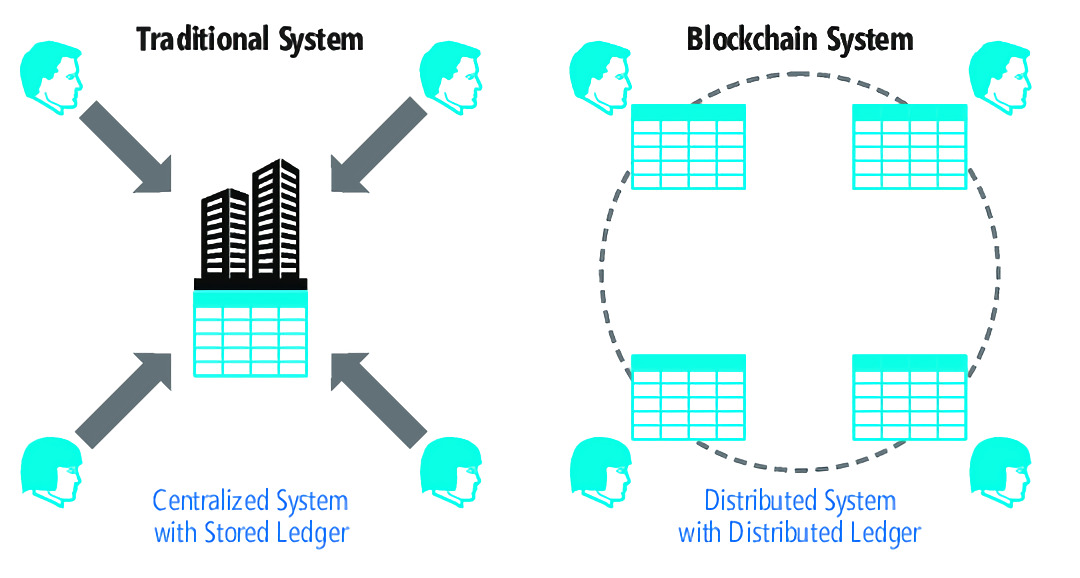
\includegraphics[width=0.70\textwidth]{dece.jpg}
		% https://docs.microsoft.com/it-it/archive/msdn-magazine/2018/july/blockchain-decentralized-applications-with-azure-blockchain-as-a-service
	\end{figure}
\end{frame}

\section{Concetti preliminari}
\begin{frame}
	\frametitle{Funzioni crittografiche di hashing}
	Funzione che \textbf{associa},
	a una qualsiasi sequenza \(m\) di lunghezza arbitraria in input, una sequenza
	in output \(h(m)\) di lunghezza costante,
	seguendo alcune proprietà che la rendono
	\emph{crittograficamente sicura}.
	Ciò impedisce di risalire all'input originale
	e facilita i \textbf{controlli di integrità sui file}.
	\begin{figure}
		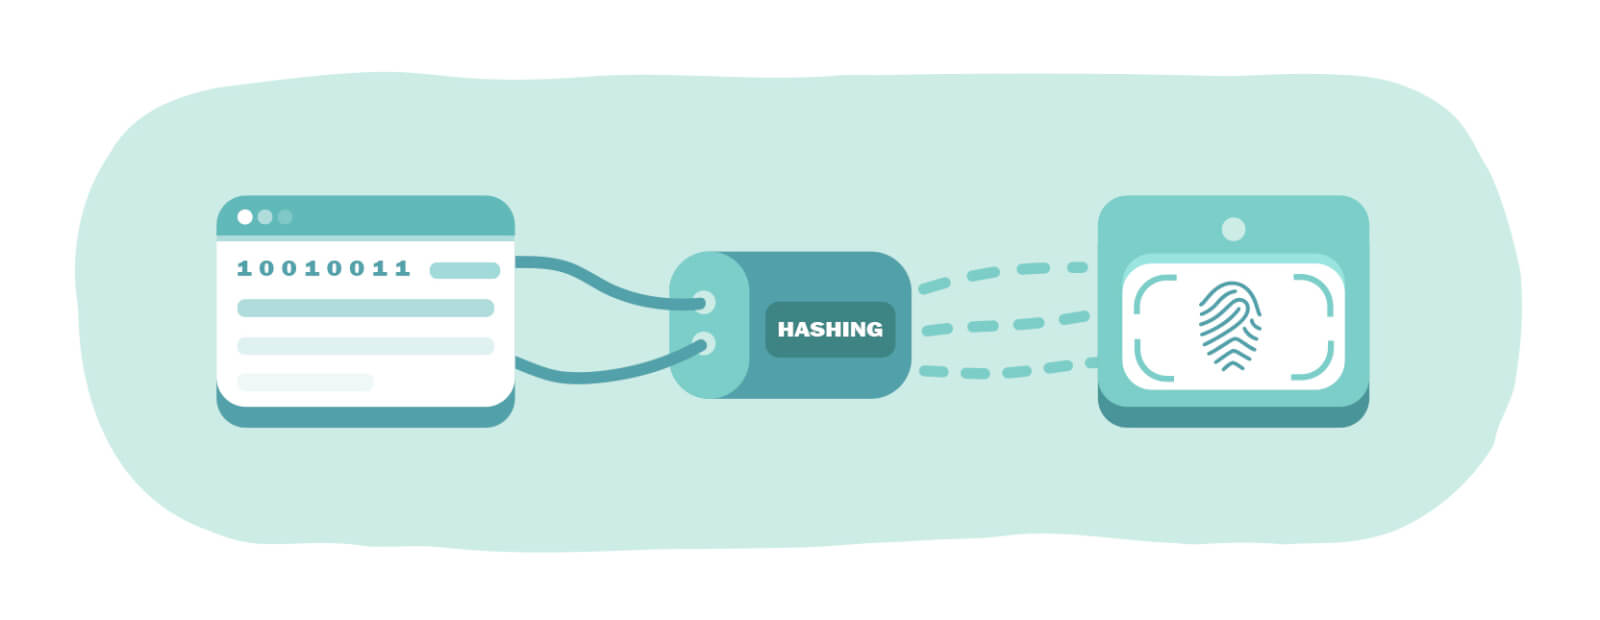
\includegraphics[width=0.85\textwidth]{figures/hashing.jpg}
	\end{figure}
\end{frame}

\begin{frame}
	\frametitle{Git}

	\begin{columns}[T]
		\column{0.99\textwidth}
		\textbf{Git} è il sistema di controllo di versione (\textbf{VCS}) \\
		distribuito più diffuso al mondo. \\
		Esso agevola la gestione \textbf{distribuita} di insiemi\\di file e directory.
		Un VCS considera tali insiemi\\unità chiamate \textbf{repository}.\\
		Git ci permette di:
		\begin{itemize}
			\item \textbf{Tracciare} le modifiche in una repository.
			\item \textbf{Ripristinare} le repository ad uno stato precedente.
			\item \textbf{Condividere} le repository con il loro storico dei cambiamenti.
		\end{itemize}
		e molto altro\dots
		\column{0.01\textwidth}
		\hspace*{-2cm}
		
\includegraphics[width=2cm]{figures/git.png}
	\end{columns}

\end{frame}

\begin{frame}
	\frametitle{Blockchain}
	La \textbf{blockchain} è un registro in continua crescita di
	record chiamati blocchi, collegati l'uno all'altro come in una
	catena grazie a metodi crittografici.
	Essa è:
	\begin{itemize}
		\item \textbf{Immutabile}.
		\item \textbf{Distribuita}.
		\item \textbf{Estremamente sicura}.
	\end{itemize}
	\begin{figure}
		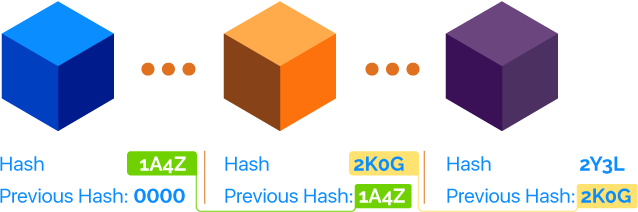
\includegraphics[width=0.65\textwidth]{figures/blockchain.png}
		% https://rubygarage.org/blog/how-blockchain-works
	\end{figure}
	\pause
	È alla base delle reti di criptovalute, come \textbf{Ethereum},
	su cui si possono anche costruire applicazioni decentralizzate con gli
	\textbf{Smart Contract}.
\end{frame}

\begin{frame}
	\frametitle{Perché blockchain?}
	L'utilizzo della blockchain nel progetto è giustificato da:
	\begin{itemize}%[<+->]
		\item Immutabilità \(\rightarrow\) Garantisce integrità dei dati
		\item Decentralizzazione \(\rightarrow\) Resistenza allo \textbf{SPOF}\footnote{Single Point Of Failure}
		\item Disintermediazione \(\rightarrow\) Eliminazione di \emph{middle-men} e dei loro costi
		\item Validazione \emph{peer-to-peer} \(\rightarrow\) Potere distribuito
	\end{itemize}
\end{frame}

\begin{frame}
	\frametitle{Il problema della blockchain}
	Vogliamo usare la blockchain per
	\textbf{immagazzinare} informazioni,
	ciò è problematico: \textbf{più dati} vorremo registrare, \textbf{più
	dovremo pagare}.
	Occorre trovare una soluzione per registrare \textbf{pochi dati}
	ma utilizzabili per \textbf{numerosi controlli} in 
	\textbf{breve tempo}.
	La soluzione è l'utilizzo di \textbf{accumulatori crittografici}.
\end{frame}

\begin{frame}
	\frametitle{Accumulatori crittografici}
	\begin{columns}
		\column{0.62\textwidth}
		Strumenti che \textbf{comprimono molte informazioni}
		in una \textbf{costante} di dimensione fissa.
		
		Un esempio ne sono i \textbf{Merkle Tree}, alberi binari
		in cui ogni foglia corrisponde all'hash di un elemento.
		Risalendo ogni nodo interno calcolerà il proprio hash
		con gli hash dei nodi figli, l'hash della root
		sarà \textbf{univoco} a quelle foglie in quell'ordine.
		\column{0.38\textwidth}
		\begin{figure}
			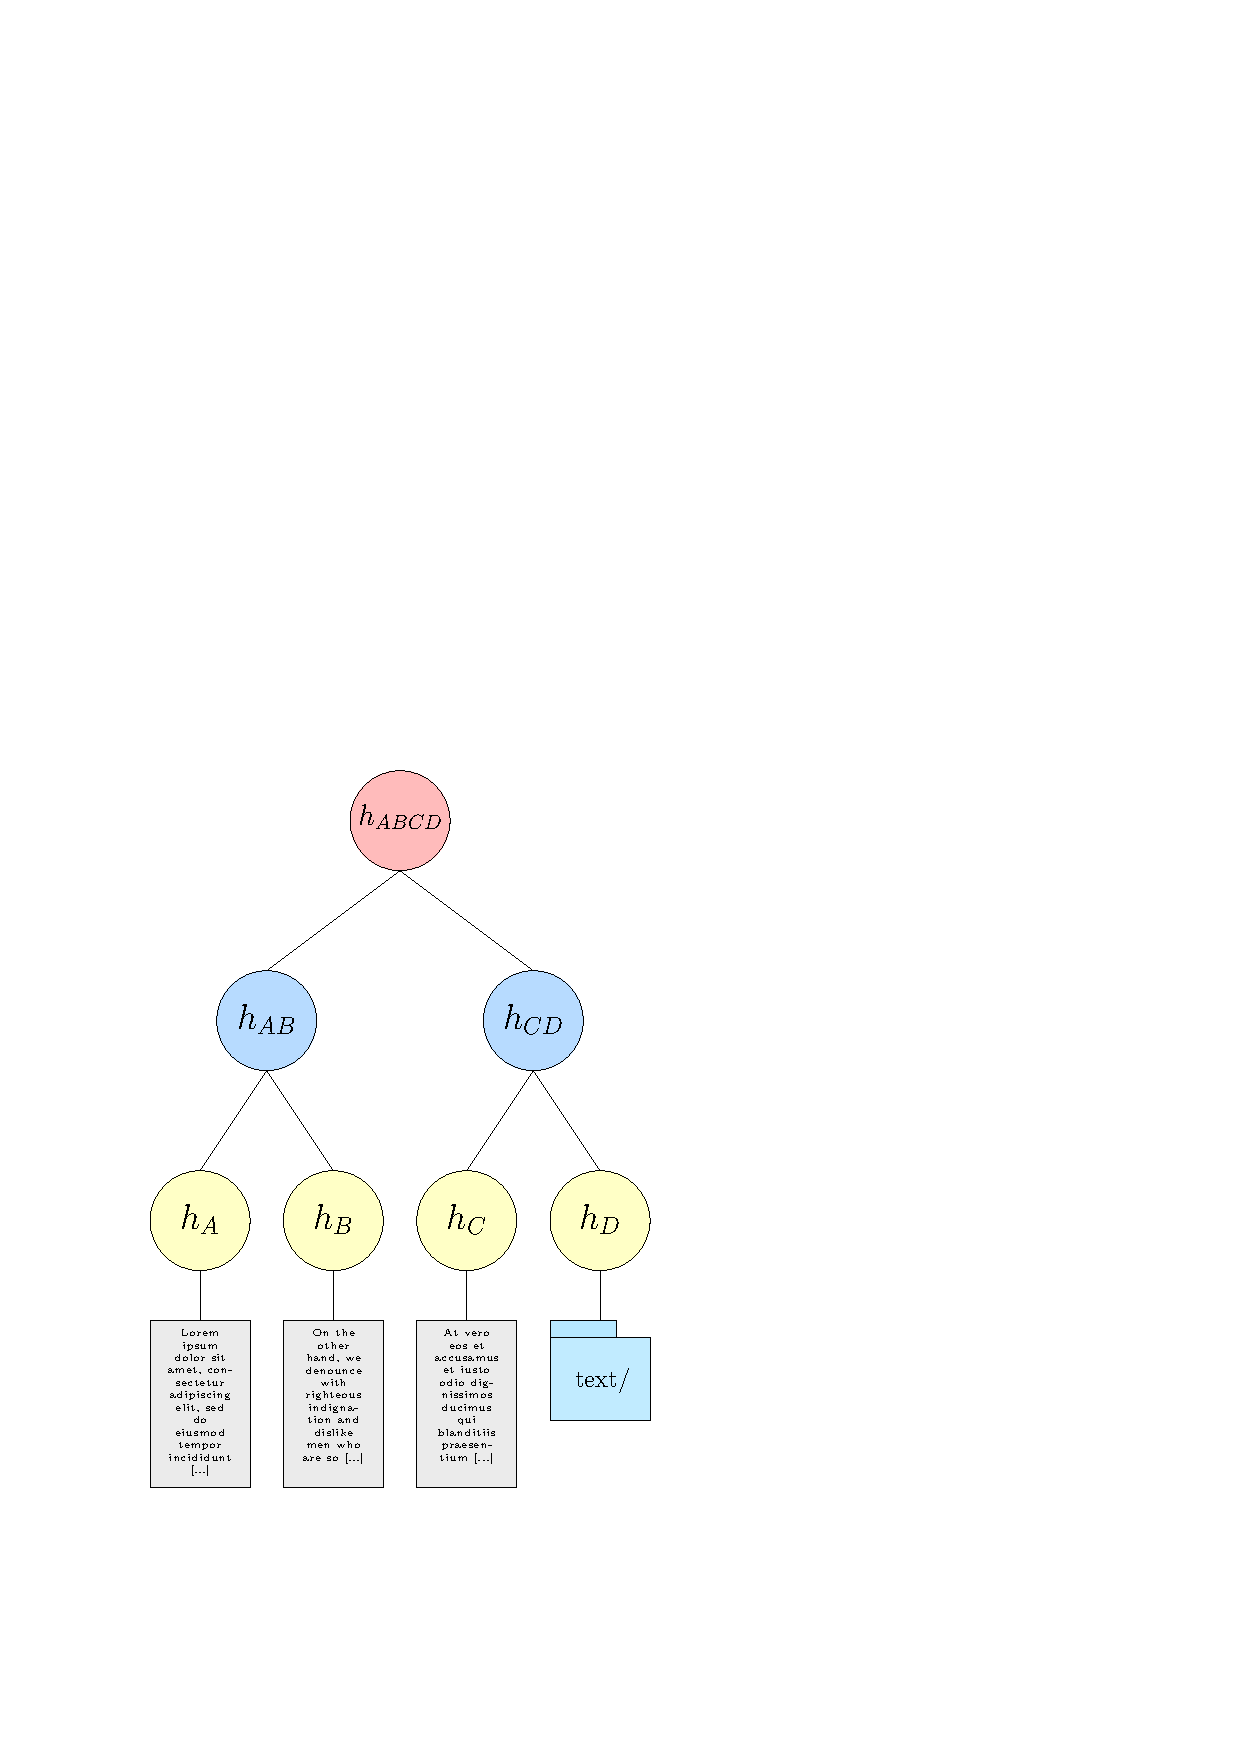
\includegraphics[width=0.9\textwidth]{figures/mt1.pdf}
		\end{figure}
	\end{columns}
\end{frame}

\section{L'Obiettivo}
\begin{frame}
	\frametitle{L'Obiettivo}
	Realizzare uno \textbf{strumento digitale distribuito} in grado, tramite
	interazioni con \textbf{Git} e la \textbf{blockchain}, di:
	\medskip
	\begin{columns}
		\column{0.33\textwidth}
		\centering
		\begin{figure}
			
\includegraphics[width=0.7\textwidth]{figures/fingerprint.png}
		\end{figure}
		\textbf{Salvare} hash di
		repository su
		blockchain
		\column{0.33\textwidth}
		\centering
		\begin{figure}
			
\includegraphics[width=0.7\textwidth]{figures/folder_zip.png}
		\end{figure}
		\textbf{Esportare} sottoinsiemi
		di repository verificabili
		\column{0.33\textwidth}
		\centering
		\begin{figure}
			
\includegraphics[width=0.7\textwidth]{figures/verify.png}
		\end{figure}
		\textbf{Verificare} l'integrità
		di singoli file e repository
	\end{columns}
\end{frame}

\section{Il Software PineSU}
\begin{frame}
	\frametitle{Il Software PineSU}
	\begin{columns}
		\column{0.7\textwidth}
		\textbf{PineSU} è un software \textbf{Javascript} che sfrutta il run-time \textbf{Node.js}. \\
		\smallskip
		L'applicazione crea delle \textbf{strutture} sulle repository Git chiamate
		\textbf{Storage Unit} (SU) tramite metadati. \\
		\smallskip
		Queste SU sono le unità su cui effettueremo le singole
		operazioni, eccetto la registrazione su blockchain che si svolgerà
		collettivamente con l'ausilio di accumulatori crittografici. 
		\column{0.3\textwidth}
		\centering
		\begin{figure}
			
\includegraphics[width=\textwidth]{figures/favicon.png}
		\end{figure} 
	\end{columns}
\end{frame}

\begin{frame}
	\frametitle{Workflow}
	\centering
	\begin{figure}
		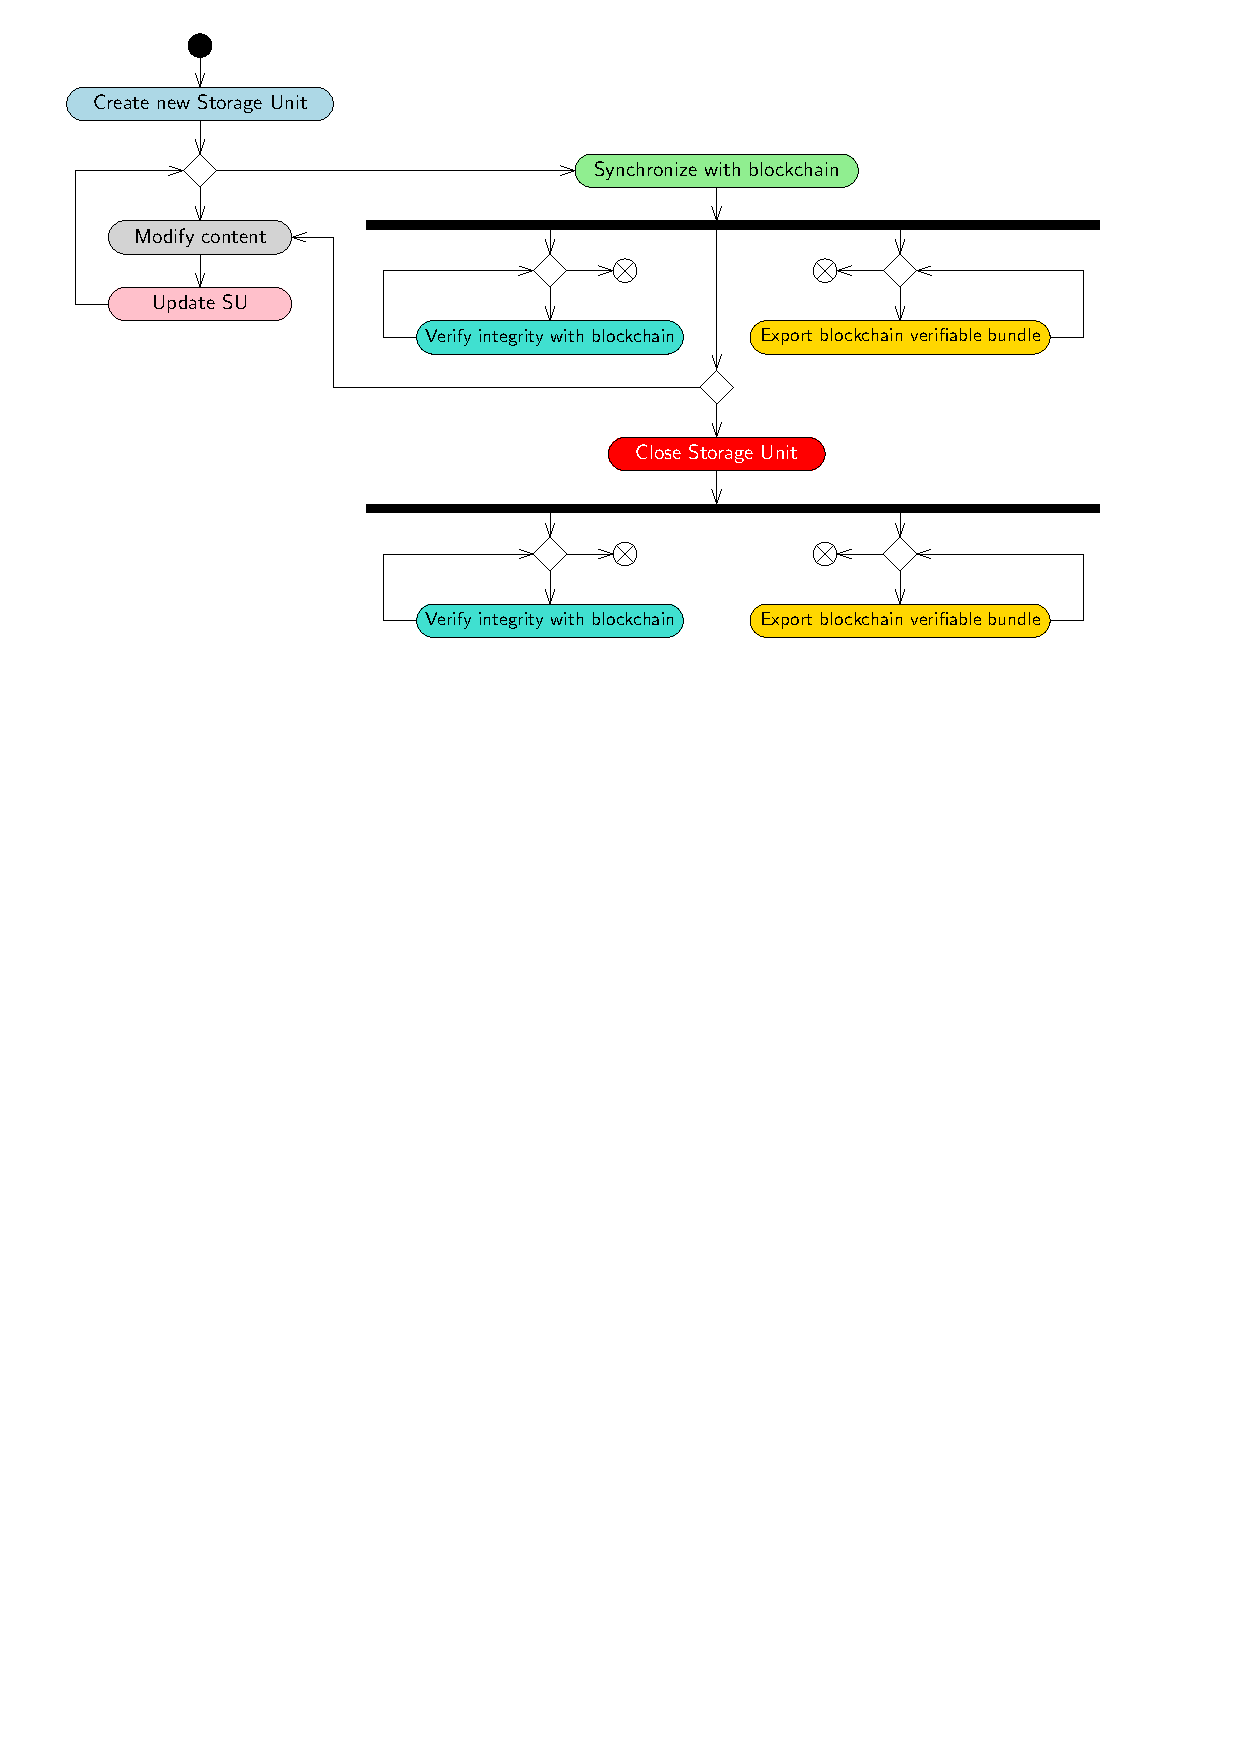
\includegraphics[width=\textwidth]{figures/activityDiag.pdf}
	\end{figure}
\end{frame}

\begin{frame}
	\frametitle{Ciclo vitale di una Storage Unit}
	\centering
	\begin{figure}
		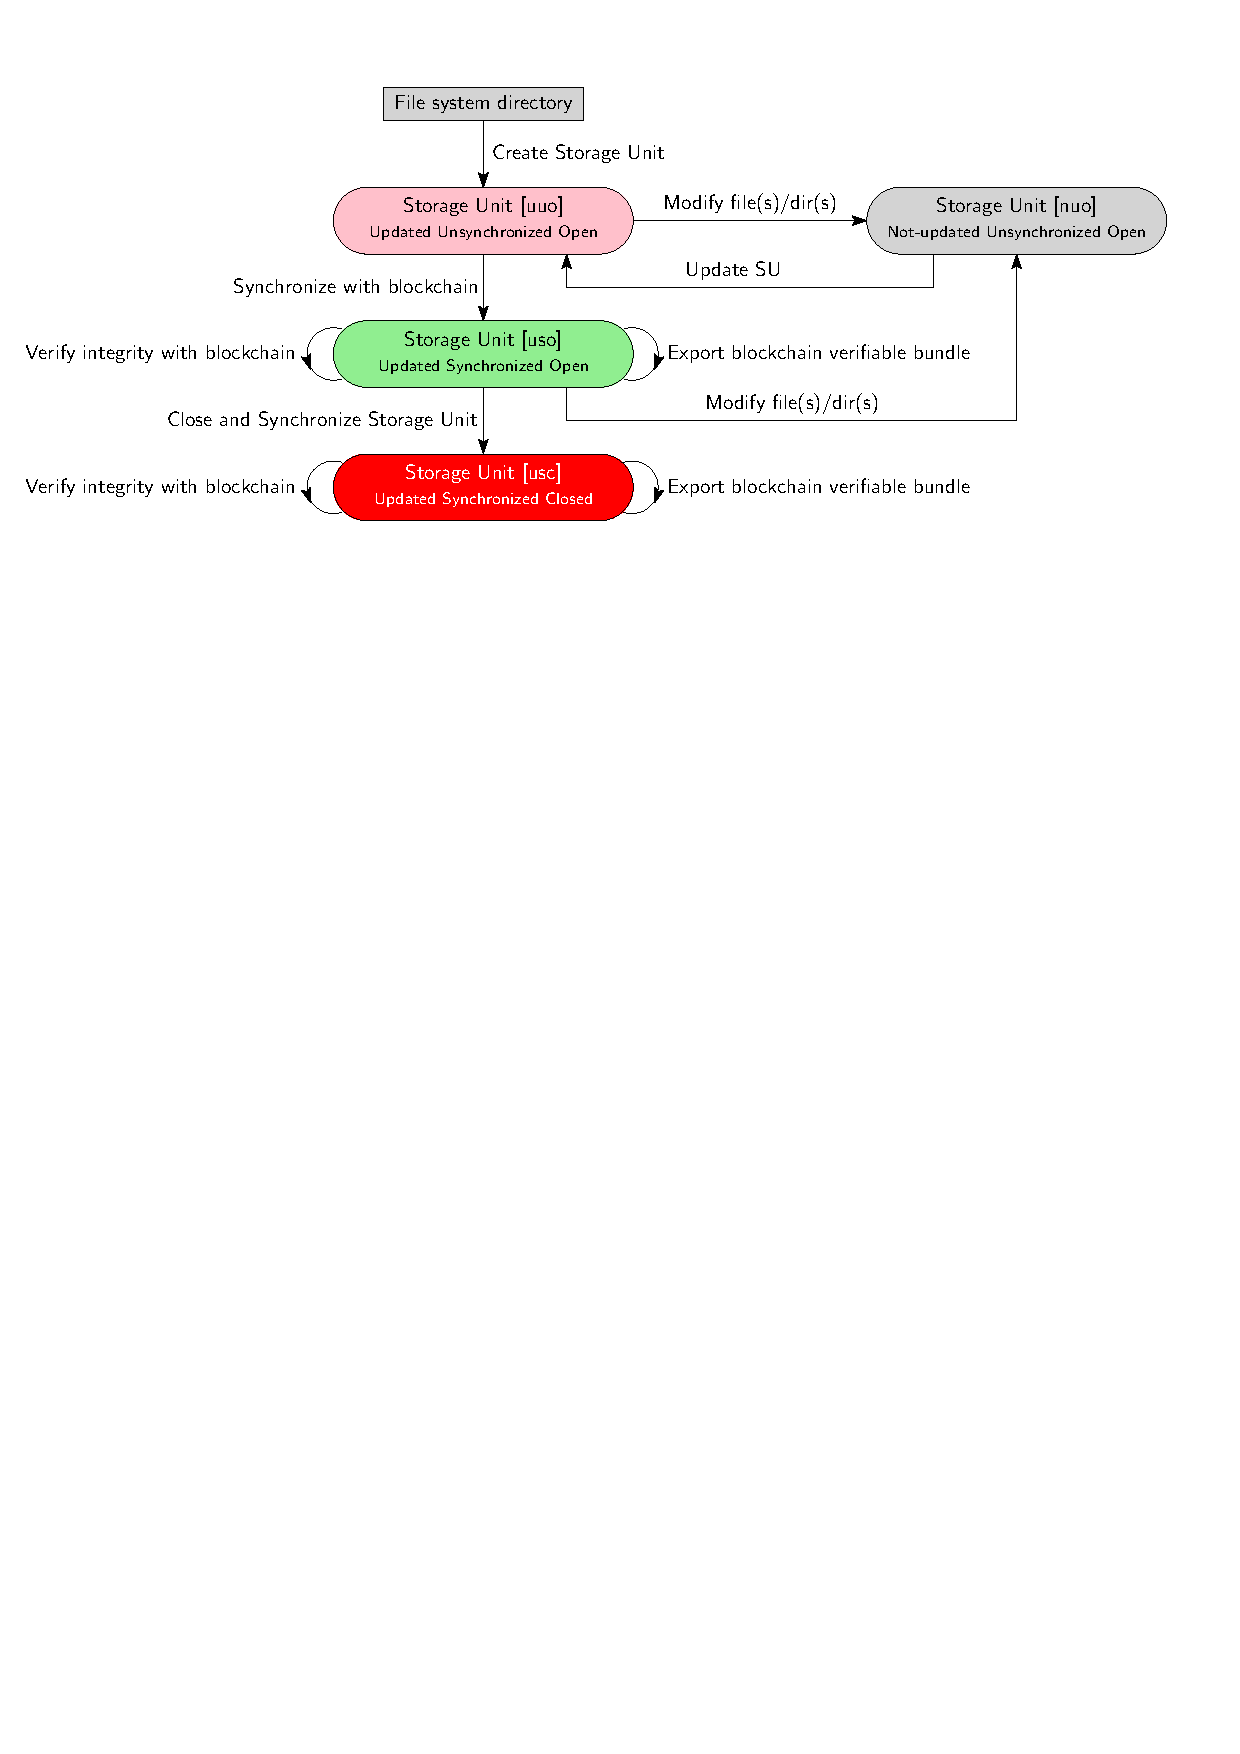
\includegraphics[width=\textwidth]{figures/stateDiag2.pdf}
	\end{figure}
\end{frame}

\begin{frame}
	\frametitle{Architettura}
	\centering
	\begin{figure}
		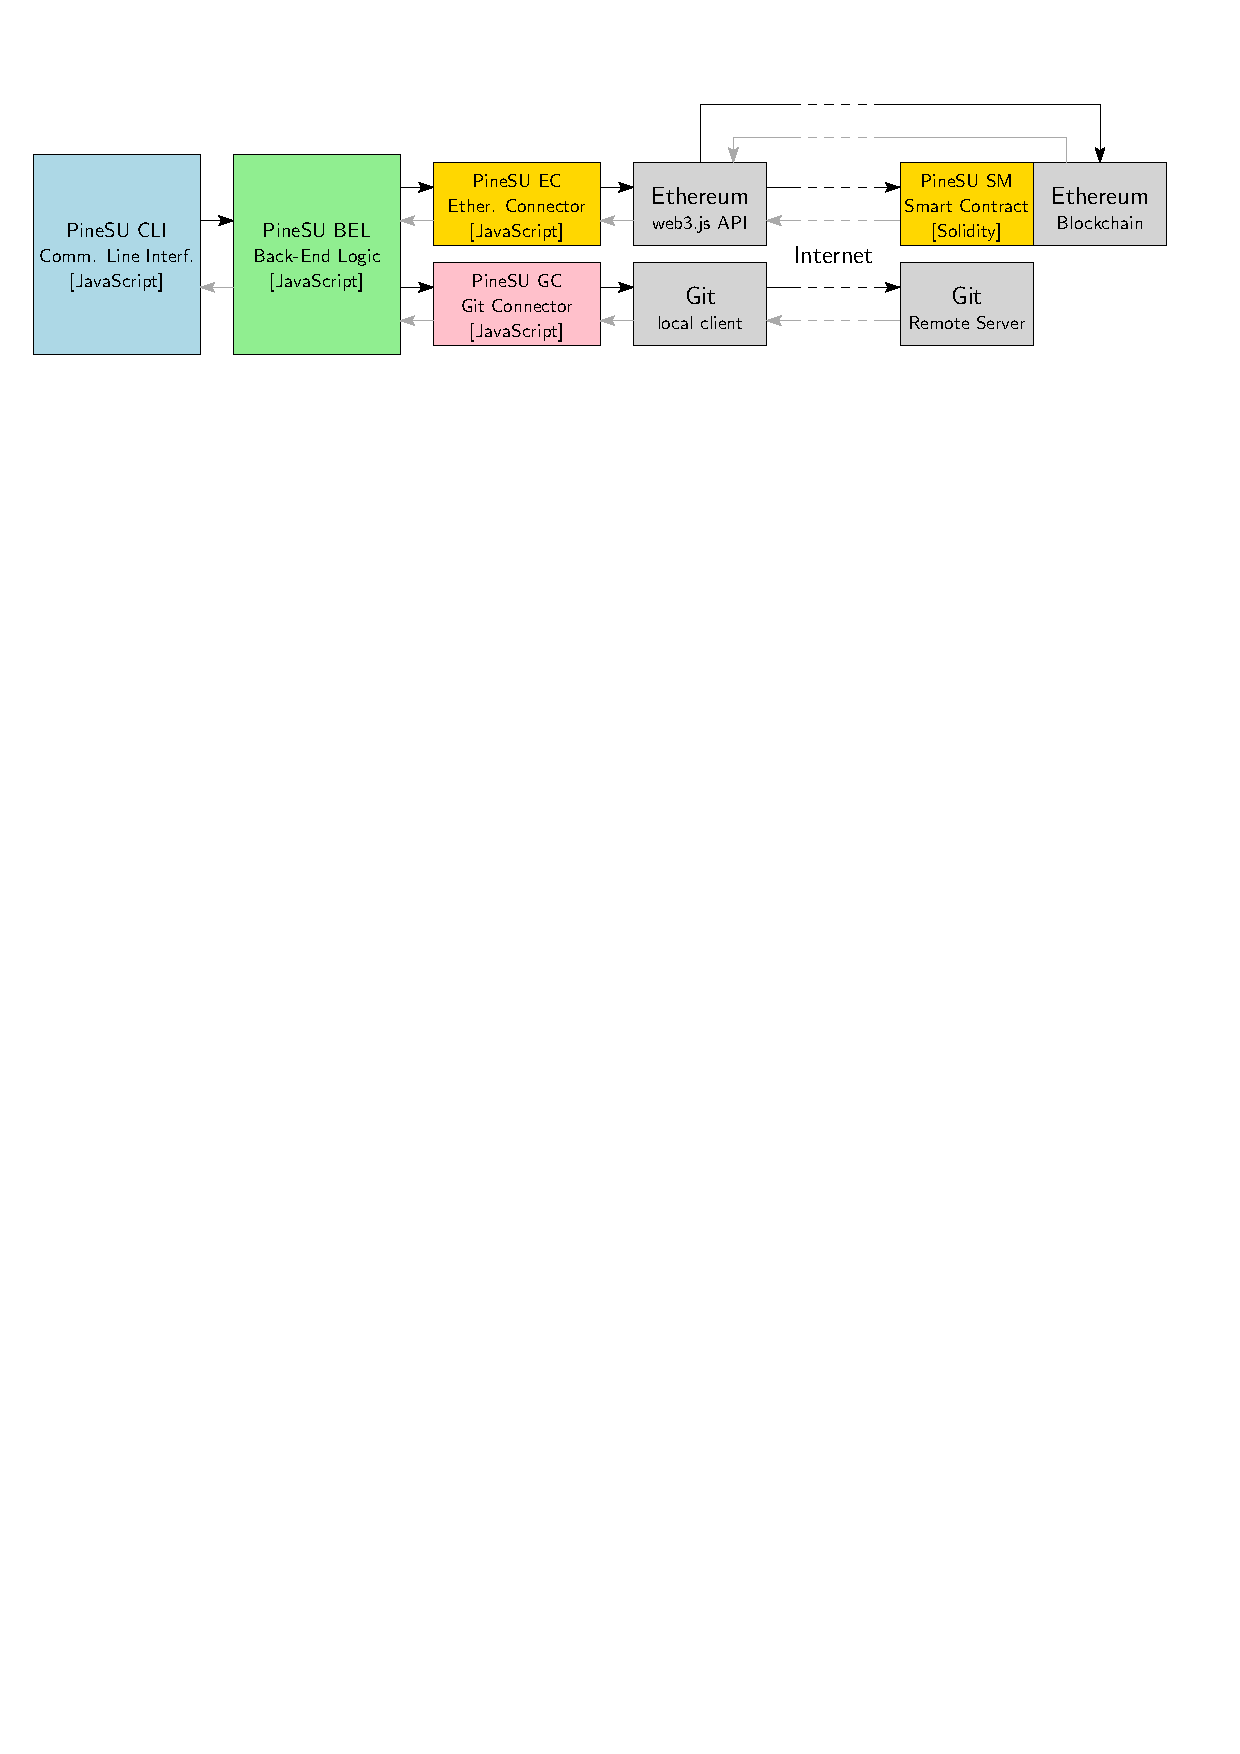
\includegraphics[width=\textwidth]{figures/pineSU-architecture.pdf}
	\end{figure}
\end{frame}

\begin{frame}
	\frametitle{Architettura (Cont.)}
	\begin{itemize}
		\item \emph{PineSU \textbf{CLI} (Command Line Interface)}: \textbf{Crea l'interfaccia utente} con cui è possibile
			interagire e \textbf{richiama le funzioni} degli altri moduli all'occorrenza.
		\item \emph{PineSU \textbf{BEL} (Back End Logic)}: Il \textbf{nucleo} di PineSU.
		\textbf{Gestisce le SU} e controlla la comunicazione con la \textbf{blockchain} e il client \textbf{Git} locale.
		\item \emph{PineSU \textbf{EC} (Ethereum Connector)}: Si interfaccia con le \textbf{API della blockchain}. 
		\item \emph{PineSU \textbf{GC} (Git Connector)}: Si interfaccia con il client \textbf{Git}. 
		\item \emph{PineSU \textbf{SM} (Smart Contract)}: Permette \textbf{registrazioni permanenti} di singole SU nella blockchain.
	\end{itemize}
\end{frame}

\begin{frame}
	\frametitle{PineSU CLI}
	\centering
	\begin{figure}
		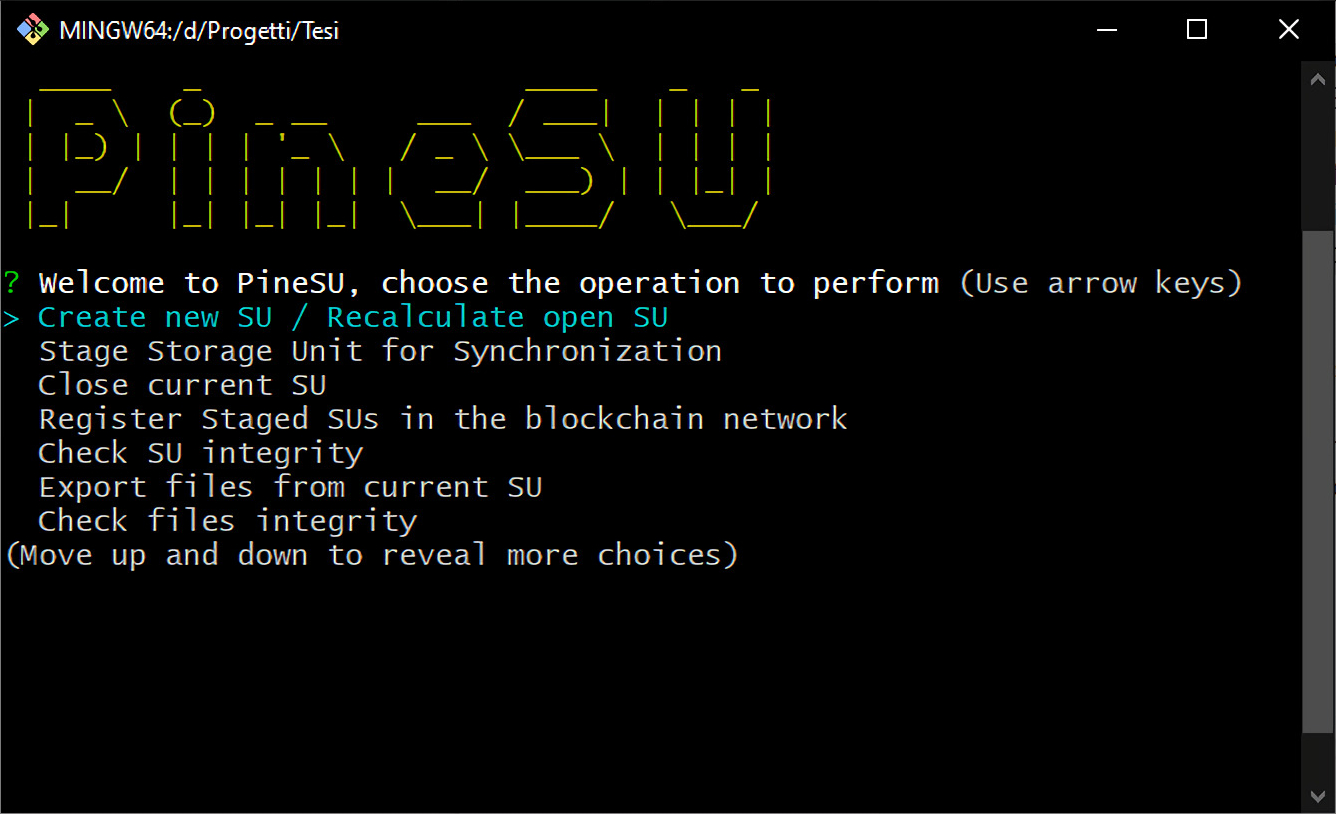
\includegraphics[width=0.95\textwidth]{figures/menu.jpg}
	\end{figure}
\end{frame}

\begin{frame}
	\frametitle{PineSU BEL}
	Il nucleo centrale che si occupa di:
	\begin{enumerate}
		\item \textbf{Gestione} dei \textbf{file descrittori}.
		\item \textbf{Gestione} degli \textbf{accumulatori crittografici}.
		\item \textbf{Comunicazione} con \textbf{Git} e \textbf{blockchain}.
	\end{enumerate}
\end{frame}

\begin{frame}
	\frametitle{Gli accumulatori di PineSU}
	\begin{columns}
		\column{0.5\textwidth}
		\begin{itemize}%[<+->]
			\item \emph{SU Merkle Tree}: Le sue \textbf{foglie} sono gli \textbf{hash dei file e directory} della SU.\\La sua \textbf{root} è l'\textbf{hash della SU} stessa. 
			\item \emph{Storage Group (\textbf{SG})}: Le sue \textbf{foglie} sono le \textbf{SU da registrare} su blockchain nella prossima transazione.
		\end{itemize}
		\column{0.5\textwidth}
		\centering
		\begin{figure}
			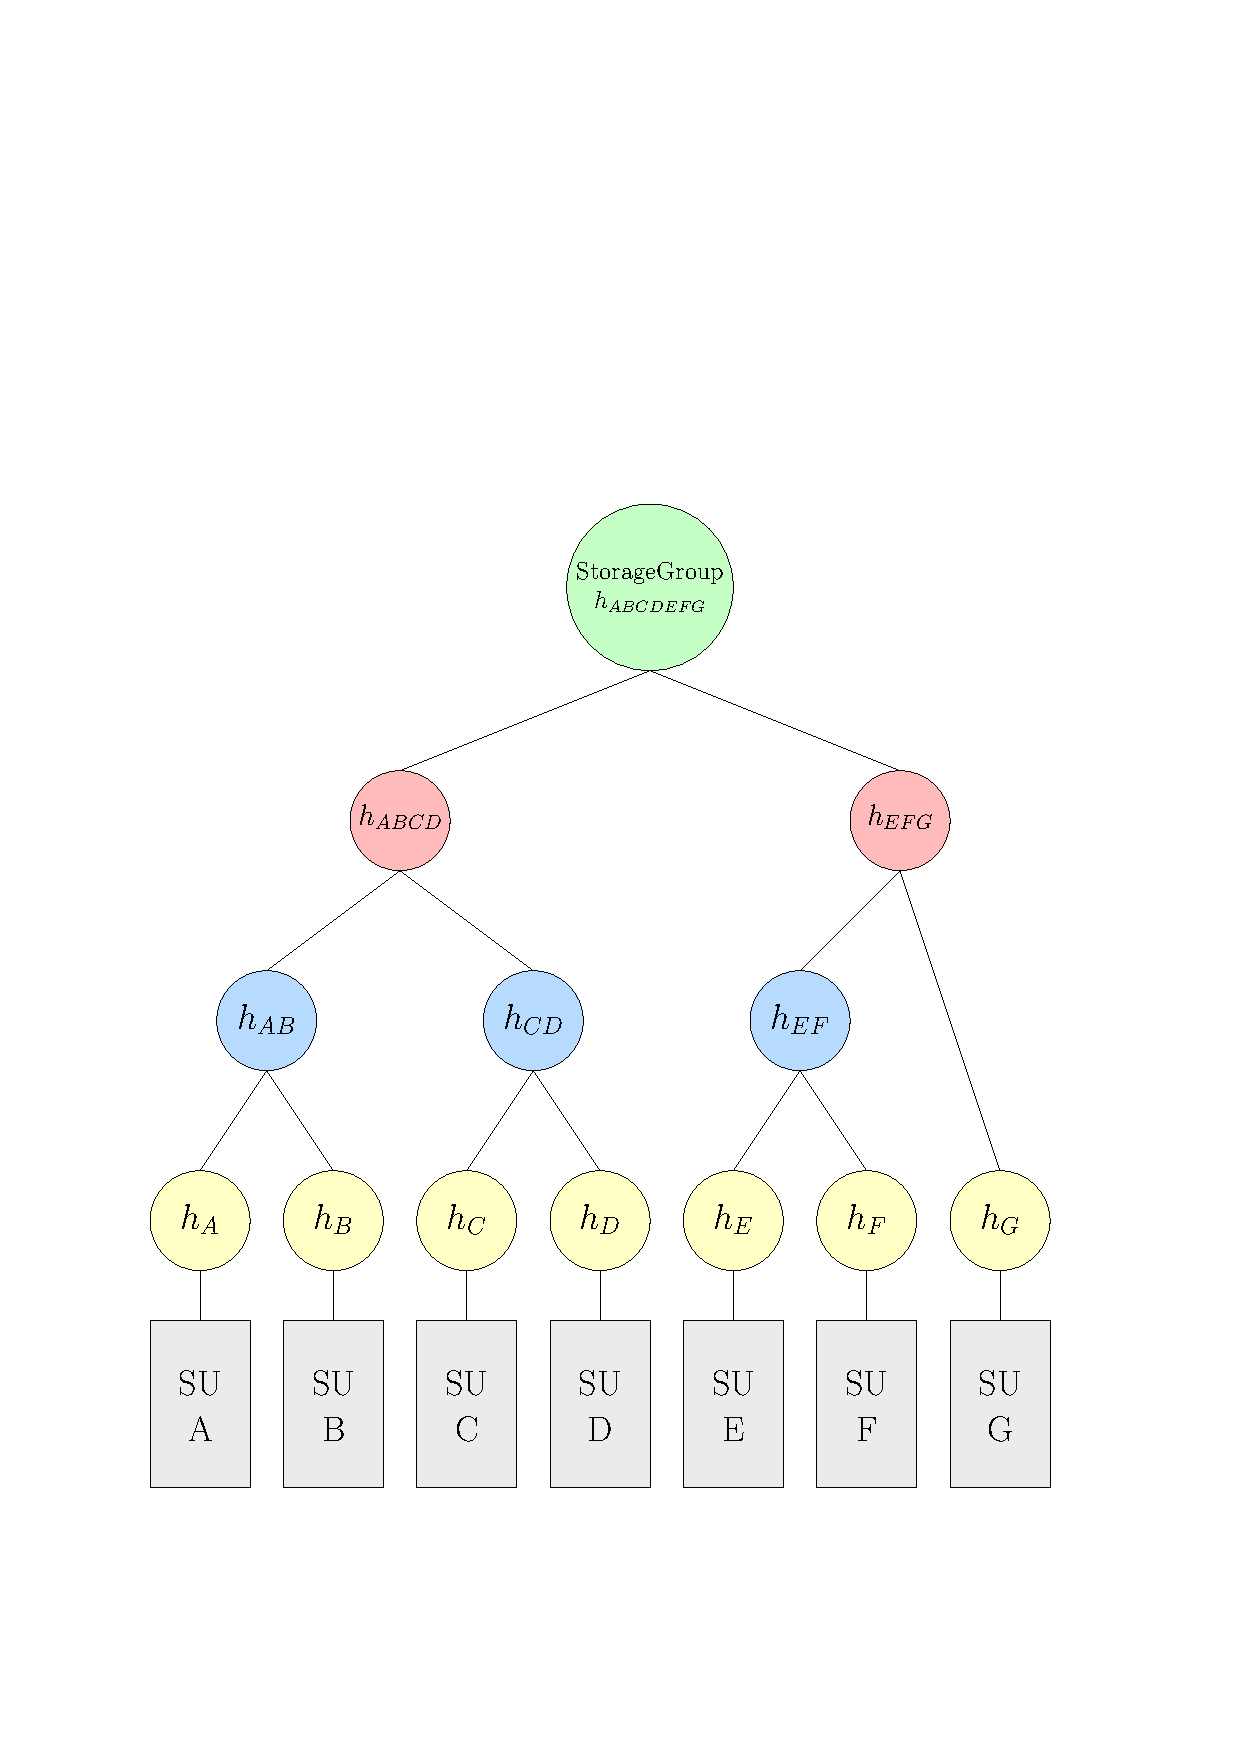
\includegraphics[width=\textwidth]{figures/sg1.pdf}
			\caption{Uno Storage Group}
		\end{figure} 
	\end{columns}
\end{frame}

\begin{frame}
	\frametitle{Gli accumulatori di PineSU (Cont.)}
	\begin{columns}
		\column{0.6\textwidth}
		\begin{itemize}
		\item \emph{Merkle Calendar (\textbf{MC})}: Albero in cui le \textbf{foglie} sono
		i Blockchain Synchronization Point (\textbf{BSP}), istanze di
		Storage Group, a loro volta raggruppate in nodi rappresentanti
		\textbf{mesi e anni}, ciò rende i reperimenti di registrazioni passate
		più agevoli e veloci.
		\end{itemize}
		\column{0.4\textwidth}
		\centering
		\begin{figure}
			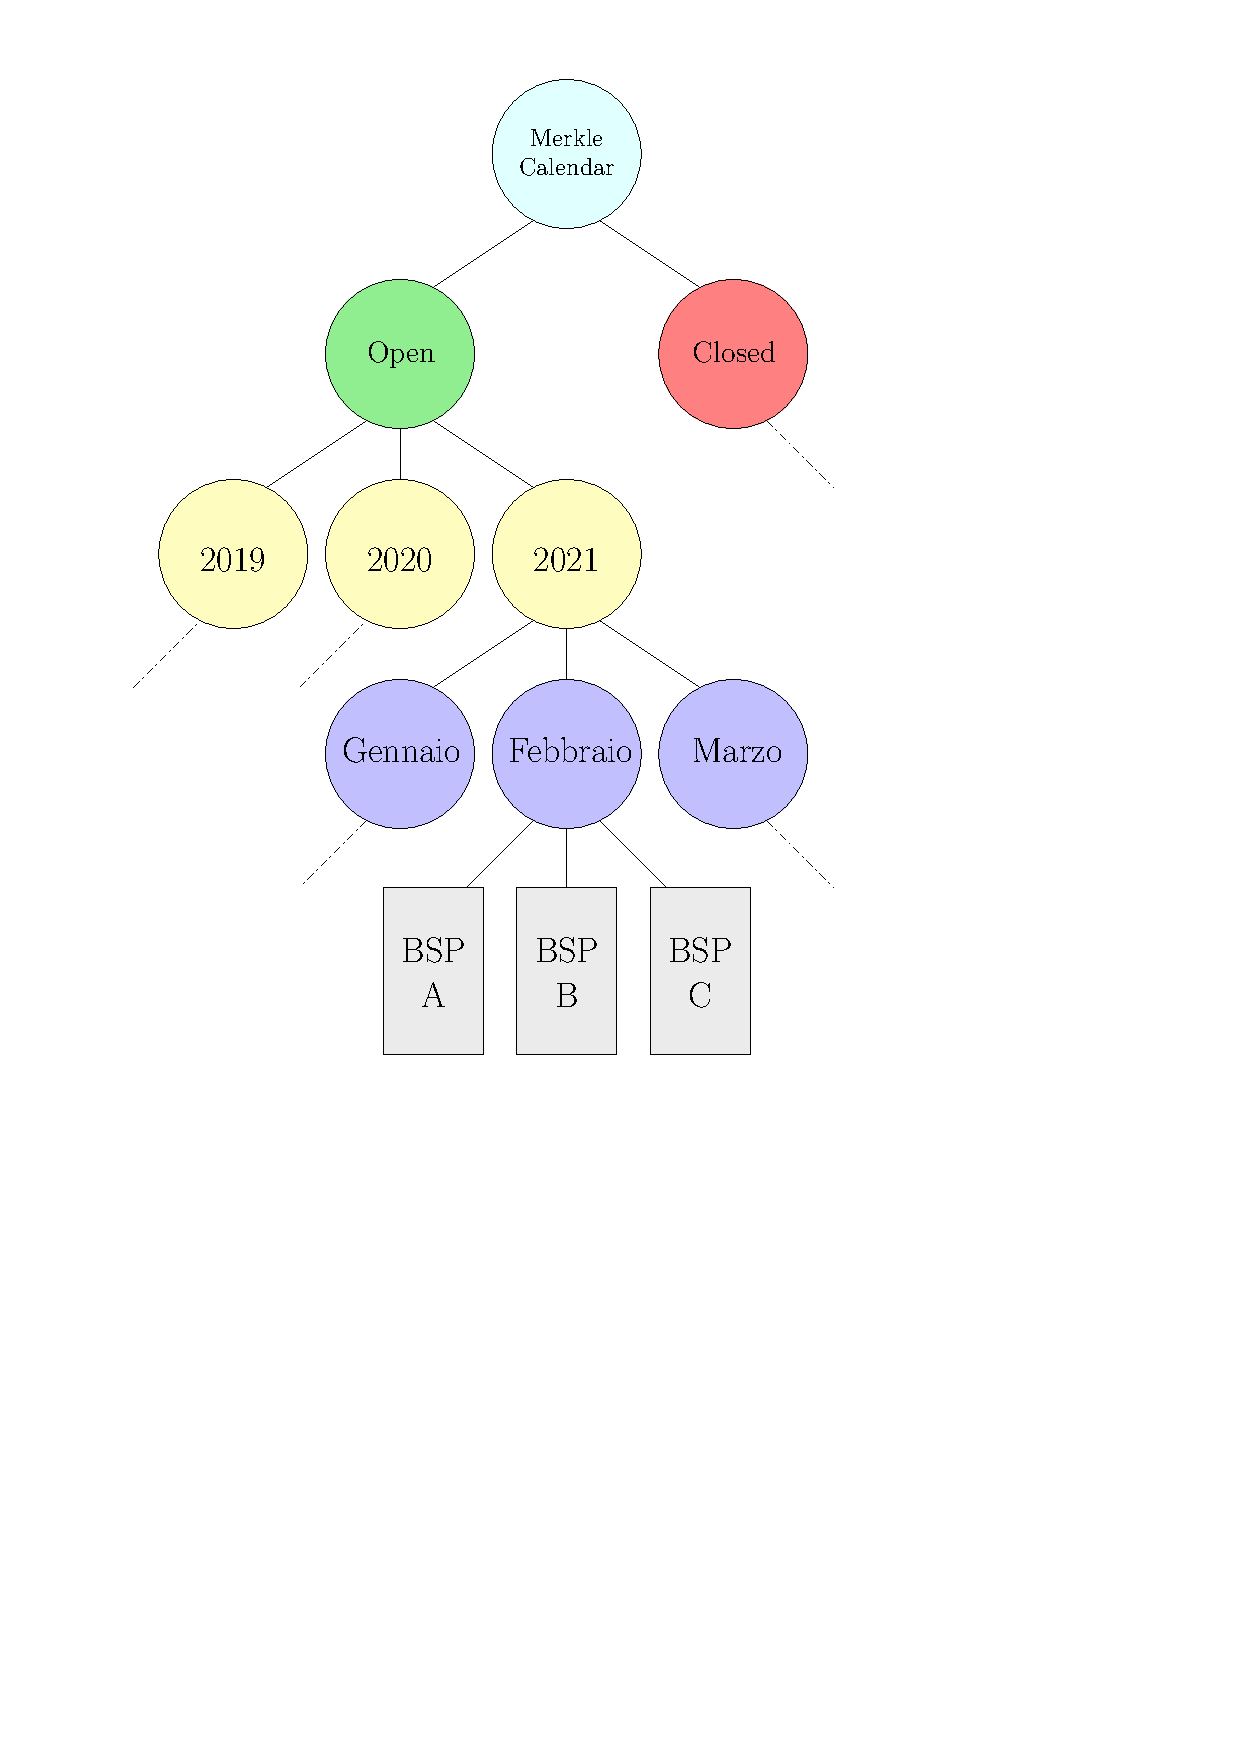
\includegraphics[width=\textwidth]{figures/mc1.pdf}
			\caption{Un Merkle Calendar}
		\end{figure} 
	\end{columns}
\end{frame}

\begin{frame}
	\frametitle{Merkle Calendar UML}
	\begin{figure}
		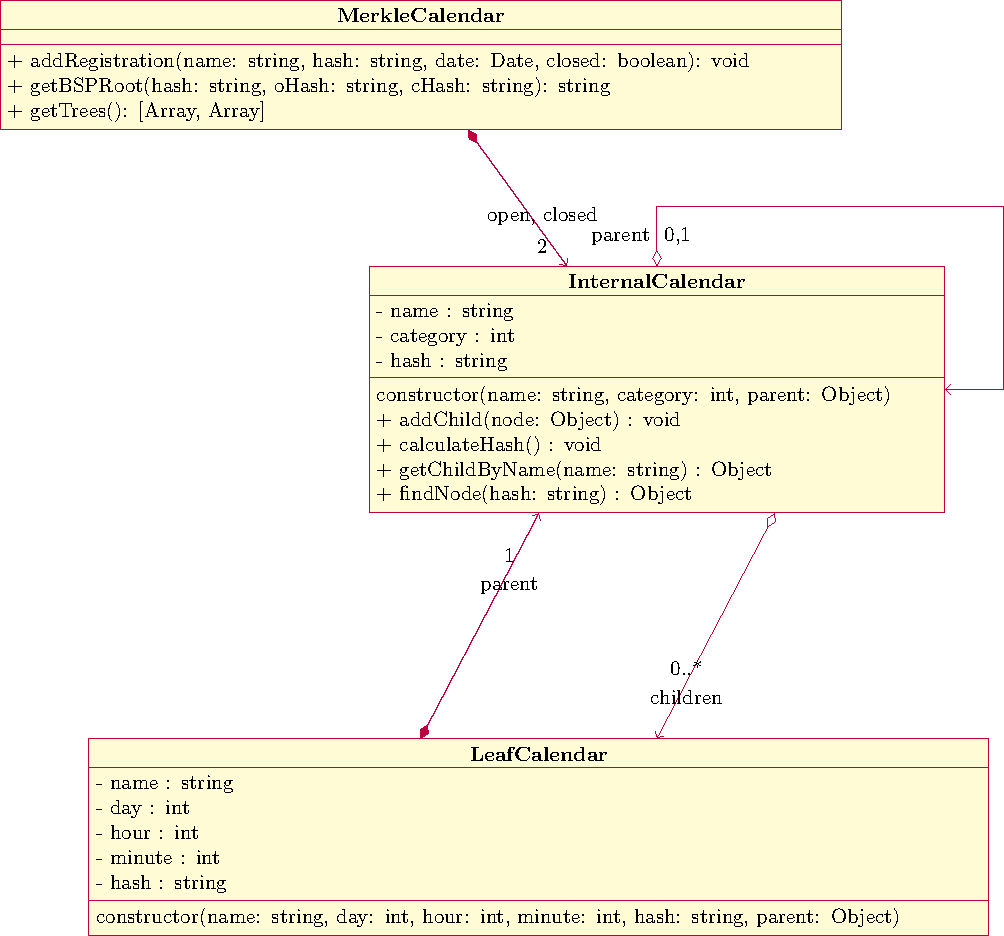
\includegraphics[width=0.75\textwidth]{figures/umlmc.pdf}
	\end{figure}
\end{frame}

\begin{frame}[fragile]
	\frametitle{Codice - Reperimento di una BSP Root}
	\begin{lstlisting}[language=JavaScript, numbers=none]
	for(let i = 0; i <= leafIndex; i++){
		leavesHash.push(monthNode.getChildByNum(i).getHash())
	}
	let newMonth = this.calculateHash(leavesHash);
	let monthsHash = new Array();
	for(let i = 0; i < monthIndex; i++){
		monthsHash.push(yearNode.getChildByNum(i).getHash())
	}
	monthsHash.push(newMonth);
	let newYear = this.calculateHash(monthsHash);
	let yearsHash = new Array();
	for(let i = 0; i < yearIndex; i++){
		yearsHash.push(yearNode.getChildByNum(i).getHash())
	}
	yearsHash.push(newYear);
	let newRoot = this.calculateHash(yearsHash)
	\end{lstlisting}
\end{frame}

\begin{frame}
	\frametitle{PineSU GC}
	\begin{figure}
		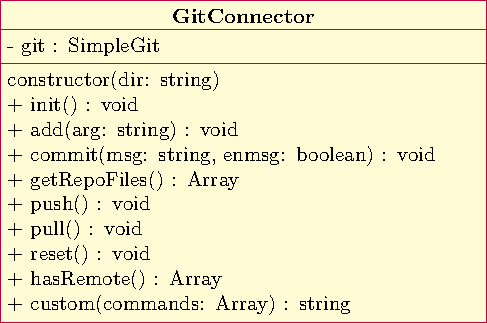
\includegraphics[width=0.85\textwidth]{figures/umlgc.pdf}
	\end{figure}
\end{frame}

\begin{frame}
	\frametitle{PineSU EC}
	\begin{figure}
		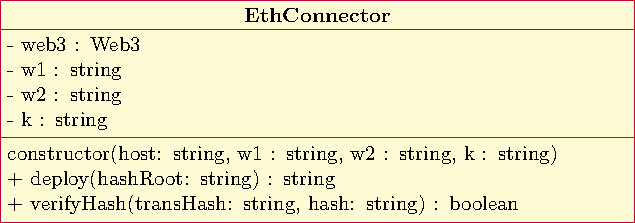
\includegraphics[width=\textwidth]{figures/umlec.pdf}
	\end{figure}
\end{frame}

\begin{frame}[fragile]
	\frametitle{Codice - Salvataggio di un hash su blockchain}
	\begin{lstlisting}[language=JavaScript, numbers=none]
	async deploy(hashRoot){
		const ct = await this.web3.eth.accounts
			.signTransaction({
				from: this.w1,
				to: this.w2,
				data: hashRoot,
				gas: 3000000,
			},
			this.k
		);
		const receipt = await this.web3.eth
			.sendSignedTransaction(ct.rawTransaction);
		return receipt.transactionHash;
	}
	\end{lstlisting}
\end{frame}

\begin{frame}[fragile]
	\frametitle{PineSU SM}
	\begin{lstlisting}[language=Solidity, numbers=none]
		contract SURegistry {
		
			string StorageUnit;
			mapping(uint => string) public registry;
			uint public SUCount;
		
			function addSU(string memory hashSU) public {
				SUCount++;
				registry[SUCount] = hashSU;
			}
		}
	\end{lstlisting}
	Codice dello \textbf{Smart Contract} che gestisce il salvataggio su blockchain delle \textbf{singole SU}.
\end{frame}

\begin{frame}
	\frametitle{Le operazioni disponibili}
	\begin{enumerate}%[<+->]
		\item Creazione di una Storage Unit o Ricalcolo di una Storage Unit pre-esistente
		\item Staging di una Storage Unit nello Storage Group
		\item Registrazione dello Storage Group nella Blockchain
		\item Chiusura di una Storage Unit
		\item Esportazione di sottoinsiemi di file da una SU
		\item Controllo di integrità di singoli file esportati da altre SU
		\item Controllo di integrità su una SU
	\end{enumerate}
\end{frame}

\begin{frame}[fragile]
	\frametitle{Creazione di una Storage Unit}
	\begin{figure}
		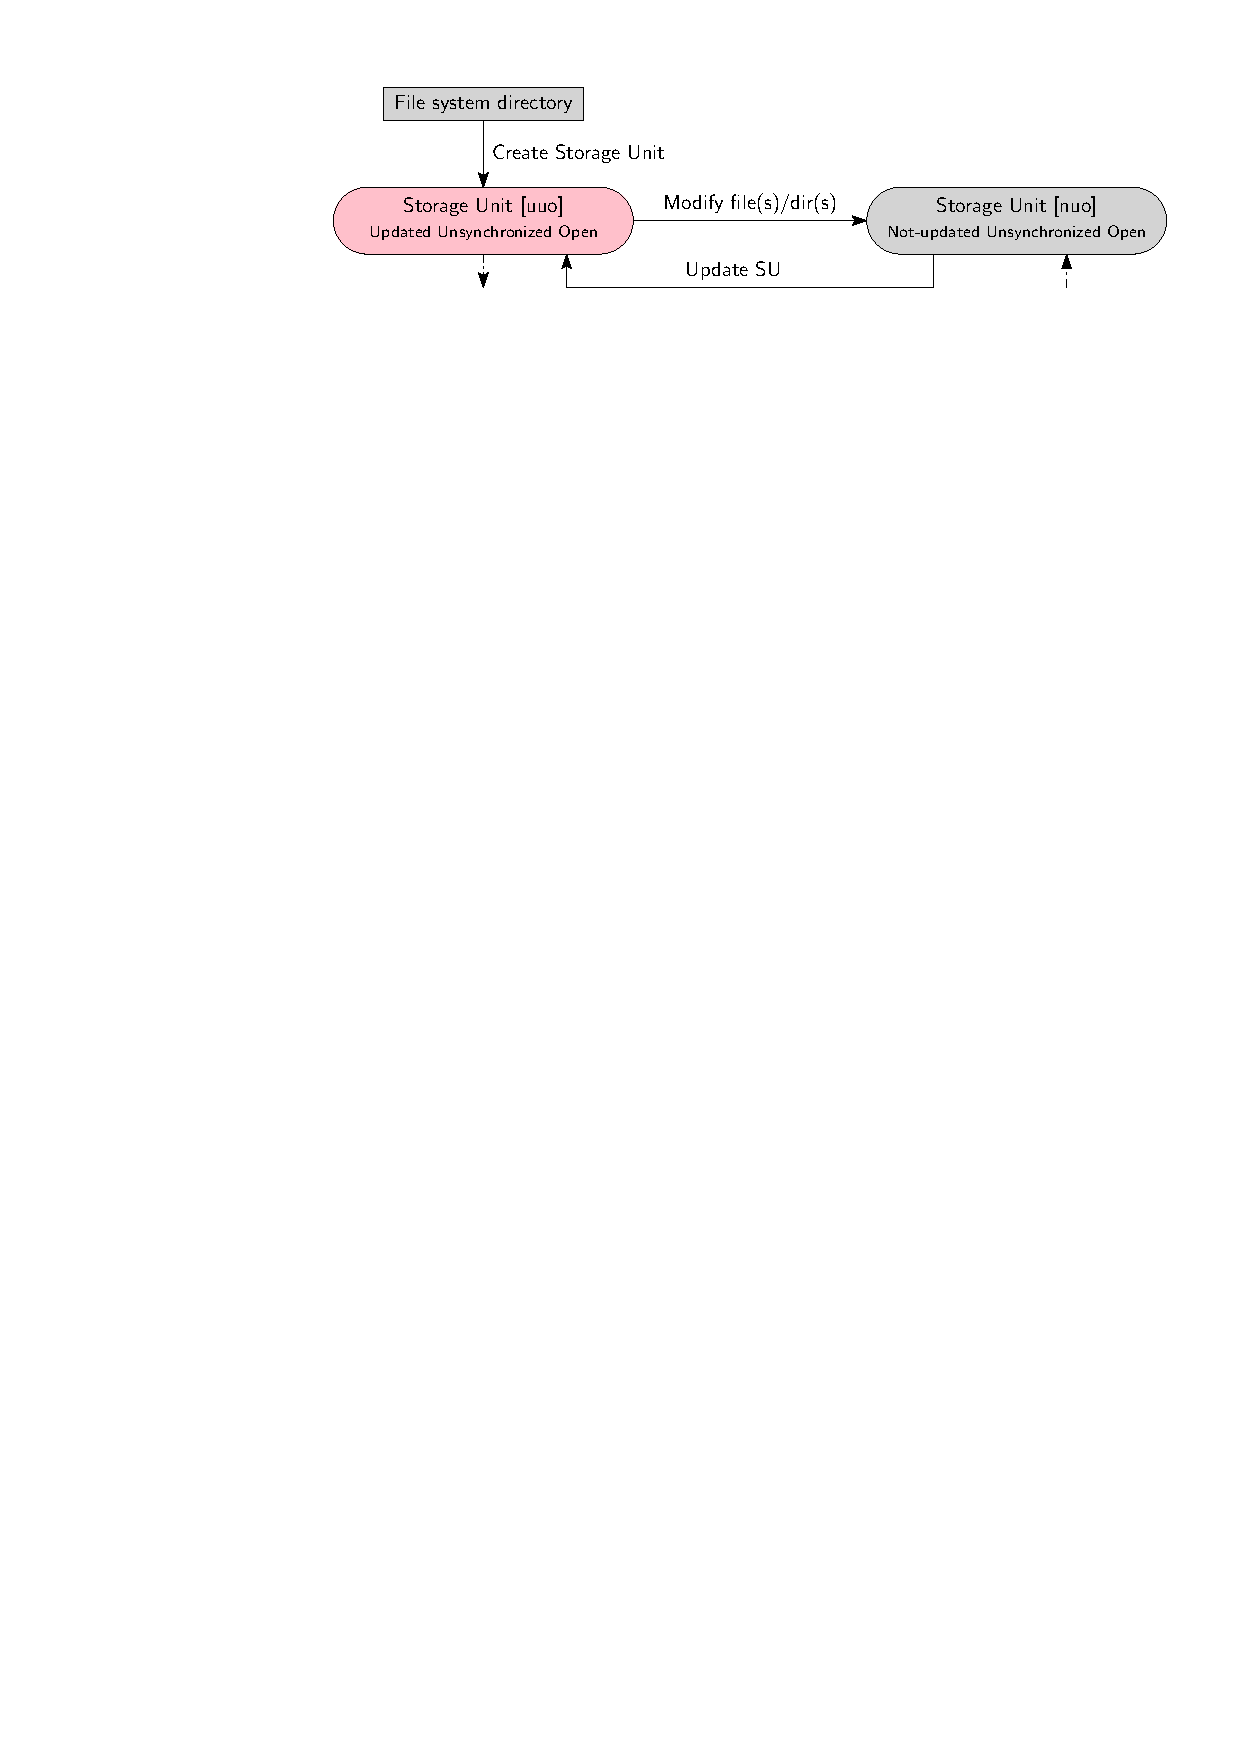
\includegraphics[width=0.8\textwidth]{figures/uuo.pdf}
	\end{figure}
	\begin{columns}
		\column{0.4\textwidth}
		\begin{figure}
			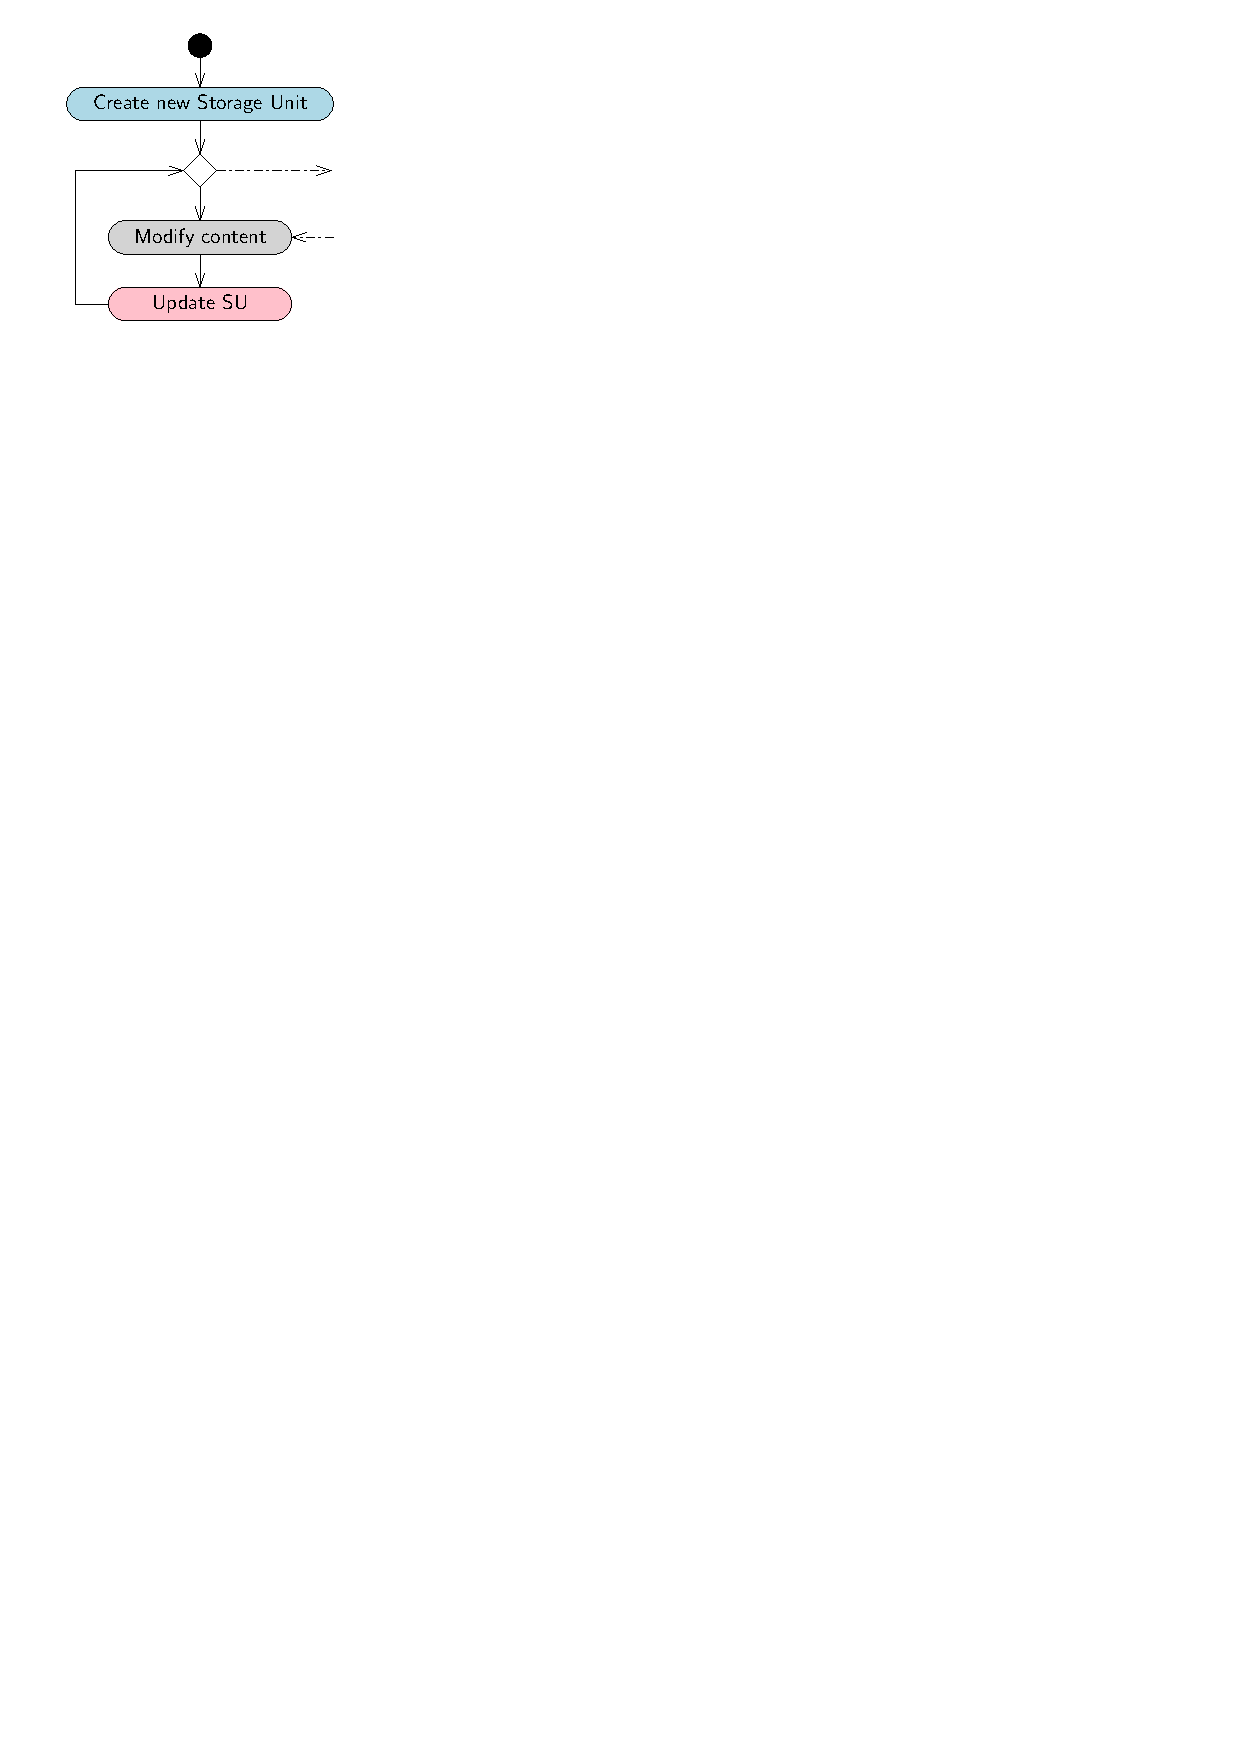
\includegraphics[width=0.8\textwidth]{figures/create.pdf}
			\bigskip
		\end{figure}
		\column{0.6\textwidth}
		\begin{lstlisting}[language=JavaScript, numbers=none]
		var merkleroot =
		 gitLogic.calculateTree(filelist);
		await inquirer.askSUDetails(
			files.getCurrentDirectoryBase(),
			remote).then((details) => {
			details.owner = w1
			details.hash = merkleroot
			details.filelist = filelist
			details.closed = false
			files.saveJSON(details);
		});
		\end{lstlisting}
	\end{columns}
\end{frame}

\begin{frame}[fragile]
	\frametitle{Registrazione di uno Storage Group}
	\begin{figure}
		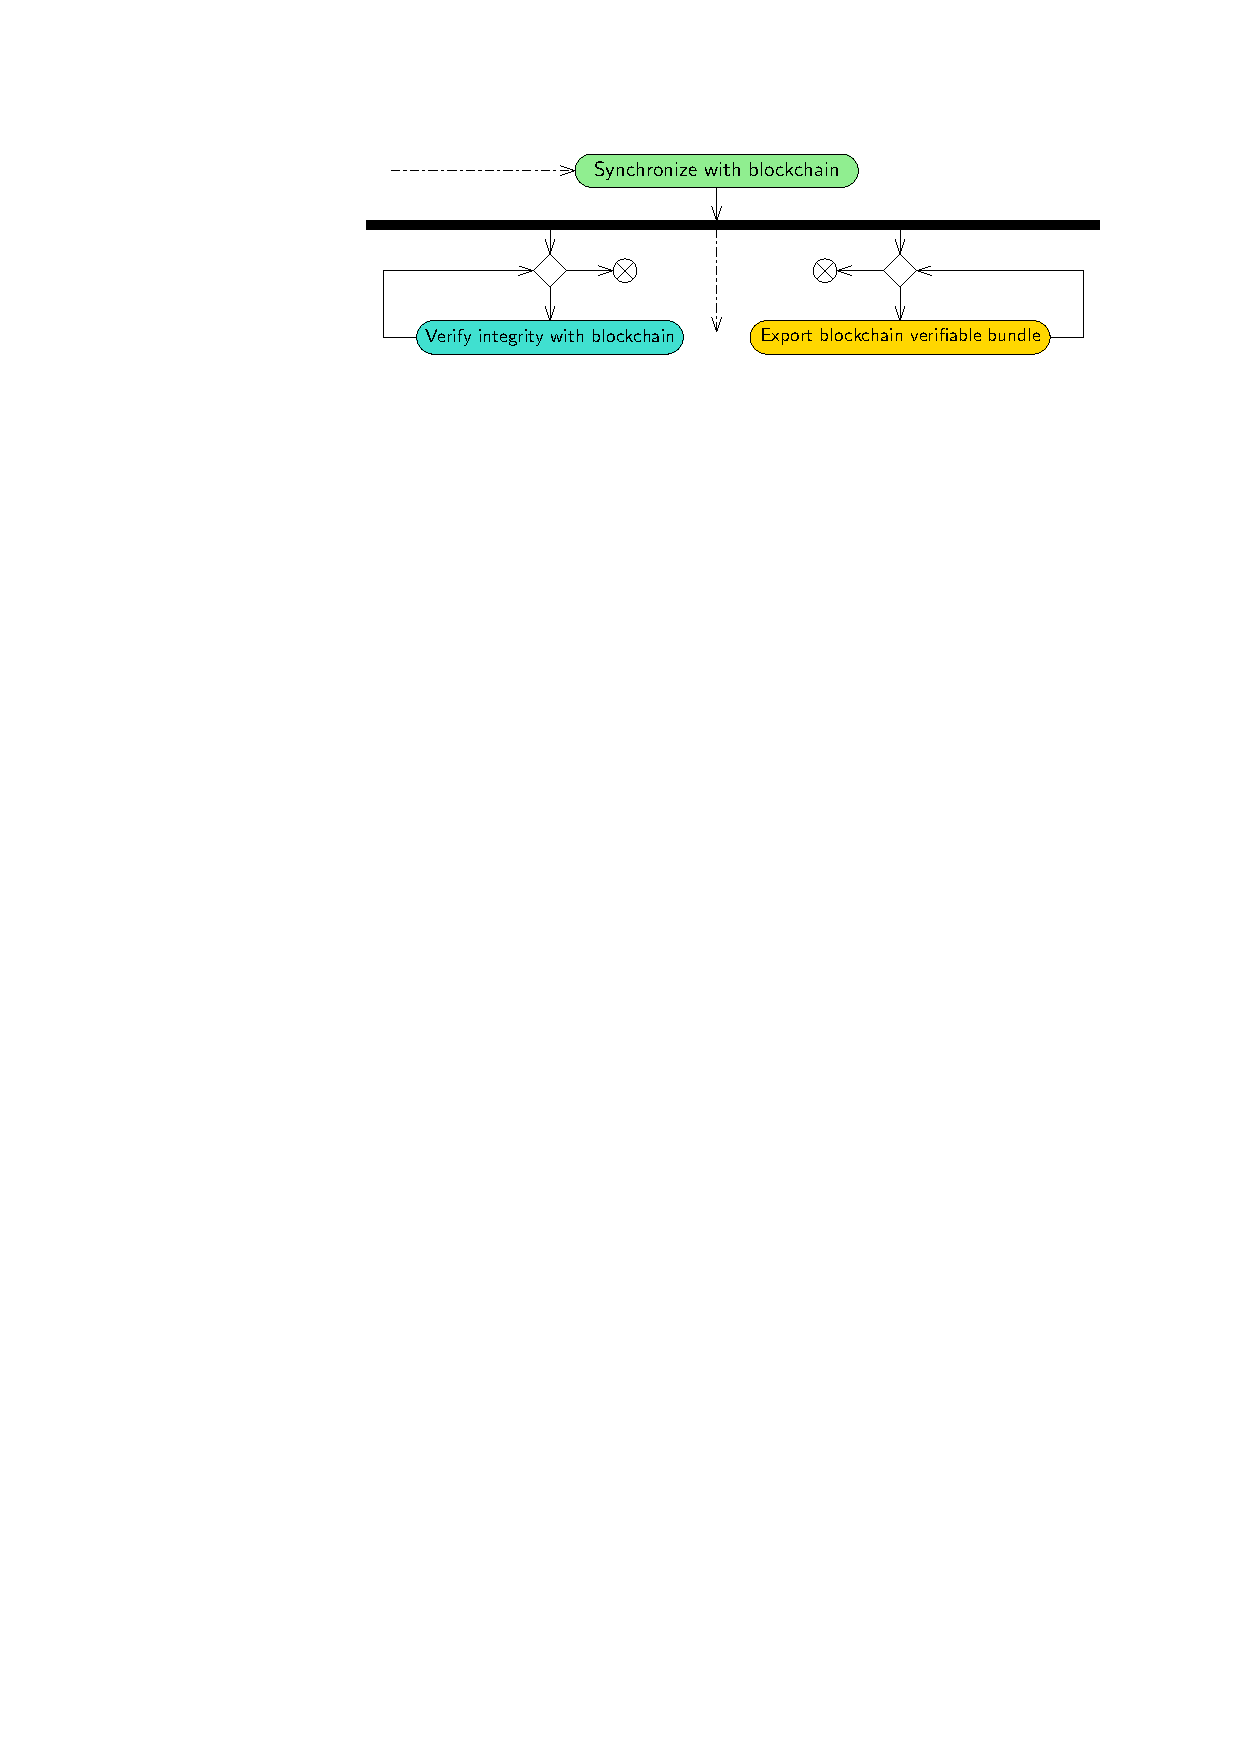
\includegraphics[width=0.8\textwidth]{figures/sync.pdf}
	\end{figure}
	\begin{columns}
		\column{0.6\textwidth}
		\begin{lstlisting}[language=JavaScript, numbers=none]
			var [doc, openRoot, closedRoot] =
				files.createSGTrees(sg);
			ethLogic.
			 addToTree(openRoot, mc, false);
			ethLogic.
			 addToTree(closedRoot, mc, true);
			var [oHash, cHash, transHash] =
			 await ethLogic.registerMC(mc);
			for(var el of document){
				el.oHash = oHash;
				el.cHash = cHash;
				el.transHash = transHash;
				files.createReg(el);
			}
		\end{lstlisting}
		\column{0.4\textwidth}
		\begin{figure}
			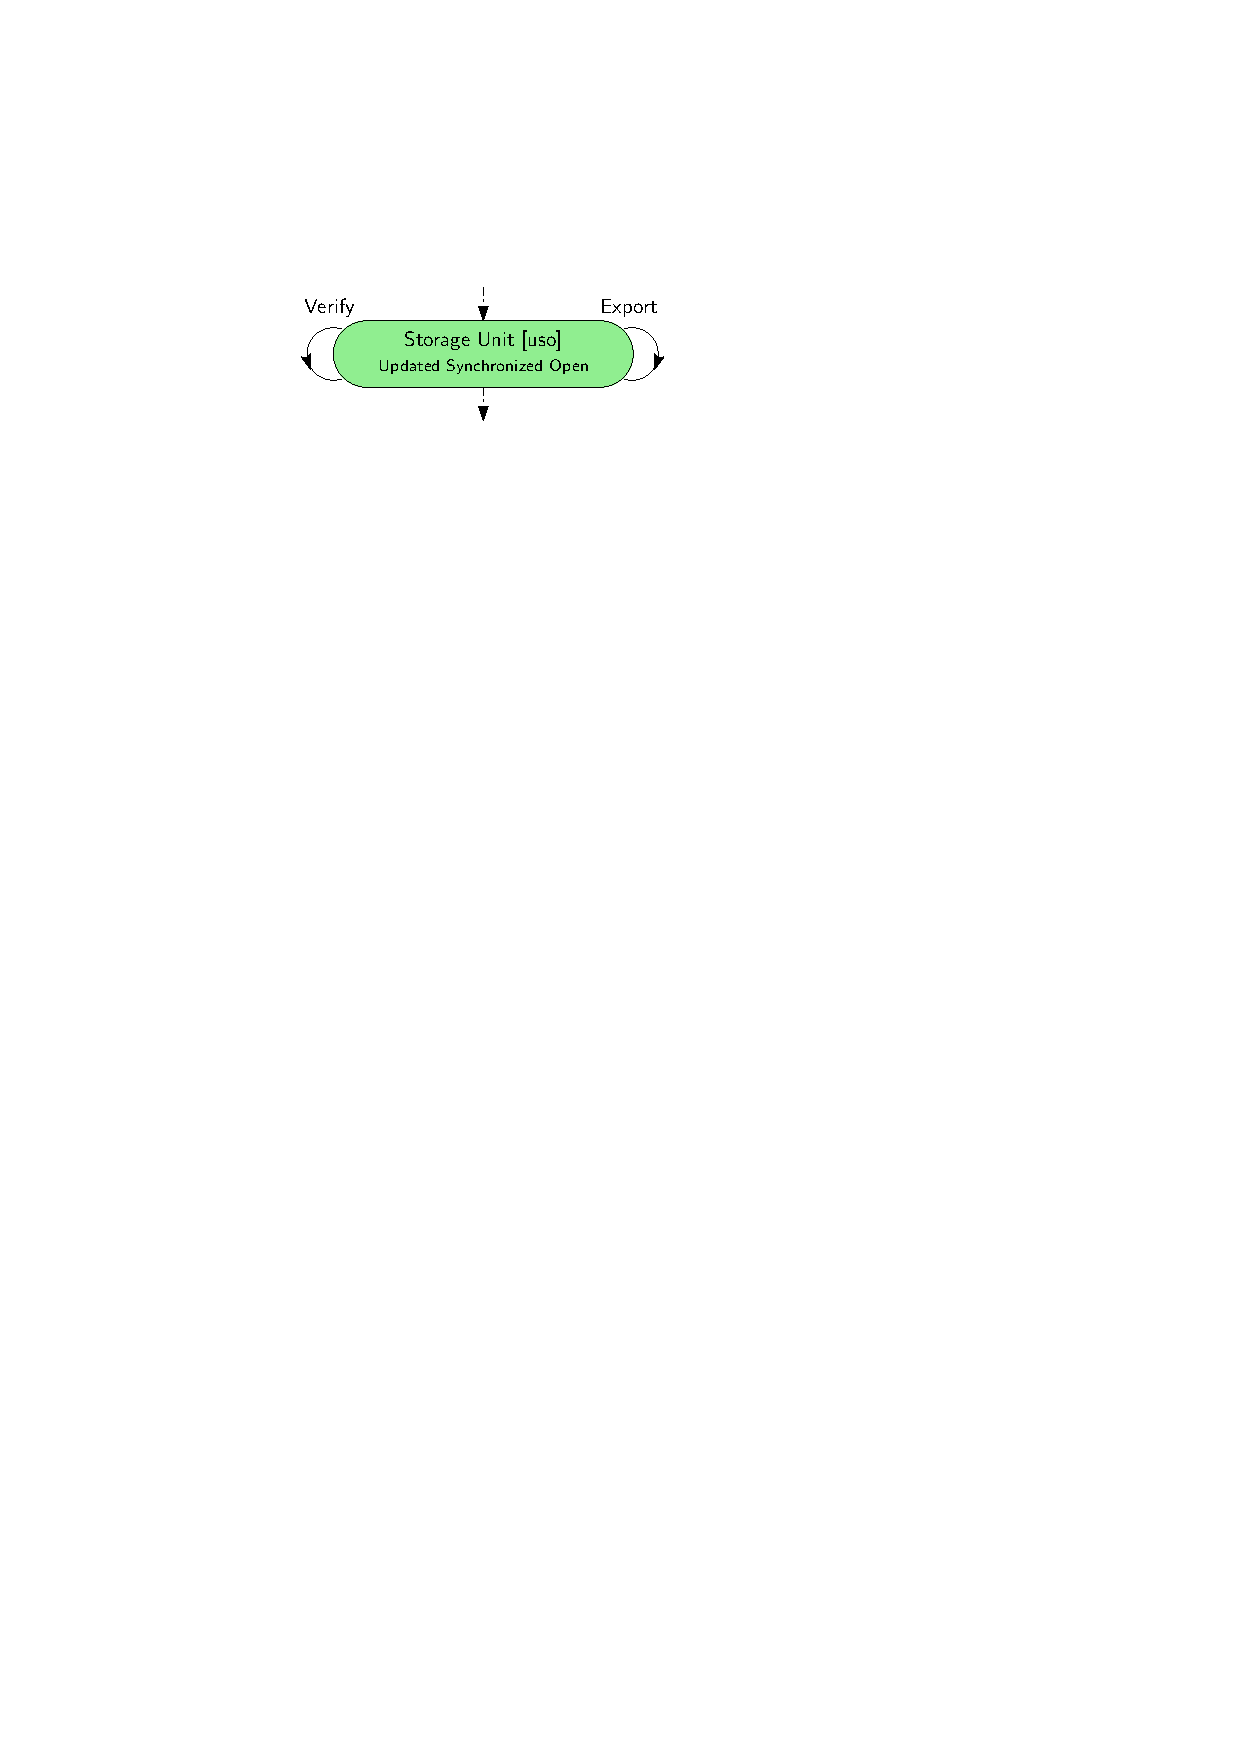
\includegraphics[width=\textwidth]{figures/uso.pdf}
			\bigskip
		\end{figure}
	\end{columns}
\end{frame}

\begin{frame}[fragile]
	\frametitle{Visualizzazione post-registrazione}
	\begin{columns}
		\column{0.5\textwidth}
		\begin{figure}
			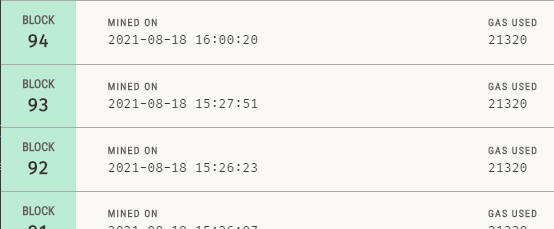
\includegraphics[width=\textwidth]{figures/blocks.png}
		\end{figure}
		\column{0.5\textwidth}
		\begin{figure}
			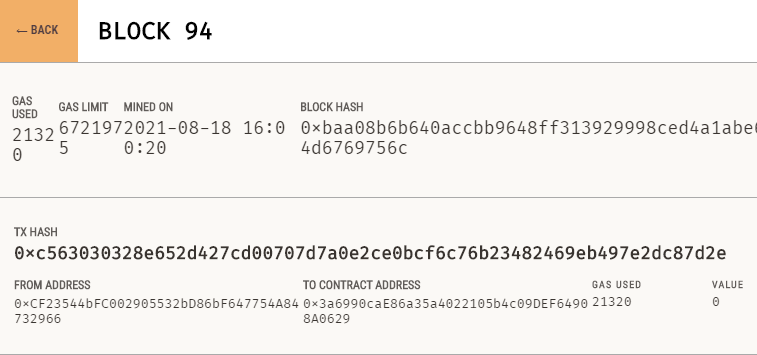
\includegraphics[width=\textwidth]{figures/block.png}
		\end{figure}
	\end{columns}
	\begin{columns}
		\column{0.5\textwidth}
		\begin{figure}
			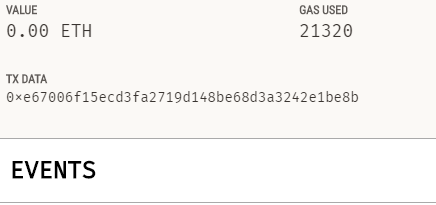
\includegraphics[width=\textwidth]{figures/block2.png}
		\end{figure}
		\bigskip
		\column{0.5\textwidth}
		\begin{lstlisting}[language=JavaScript, numbers=none]
			|\color{blue}"path"|:
				"D:/Progetti/Tirocinio/sample",
			|\color{blue}"root"|:
				"e67006f15ecd3[...]e6
				8d3a3242e1be8b",
			|\color{blue}"transHash"|:
				"0xc563030328e[...]69eb497e2dc87d2e"
		\end{lstlisting}
	\end{columns}
\end{frame}

\begin{frame}[fragile]
	\frametitle{Chiusura di una Storage Unit}
	\begin{figure}
		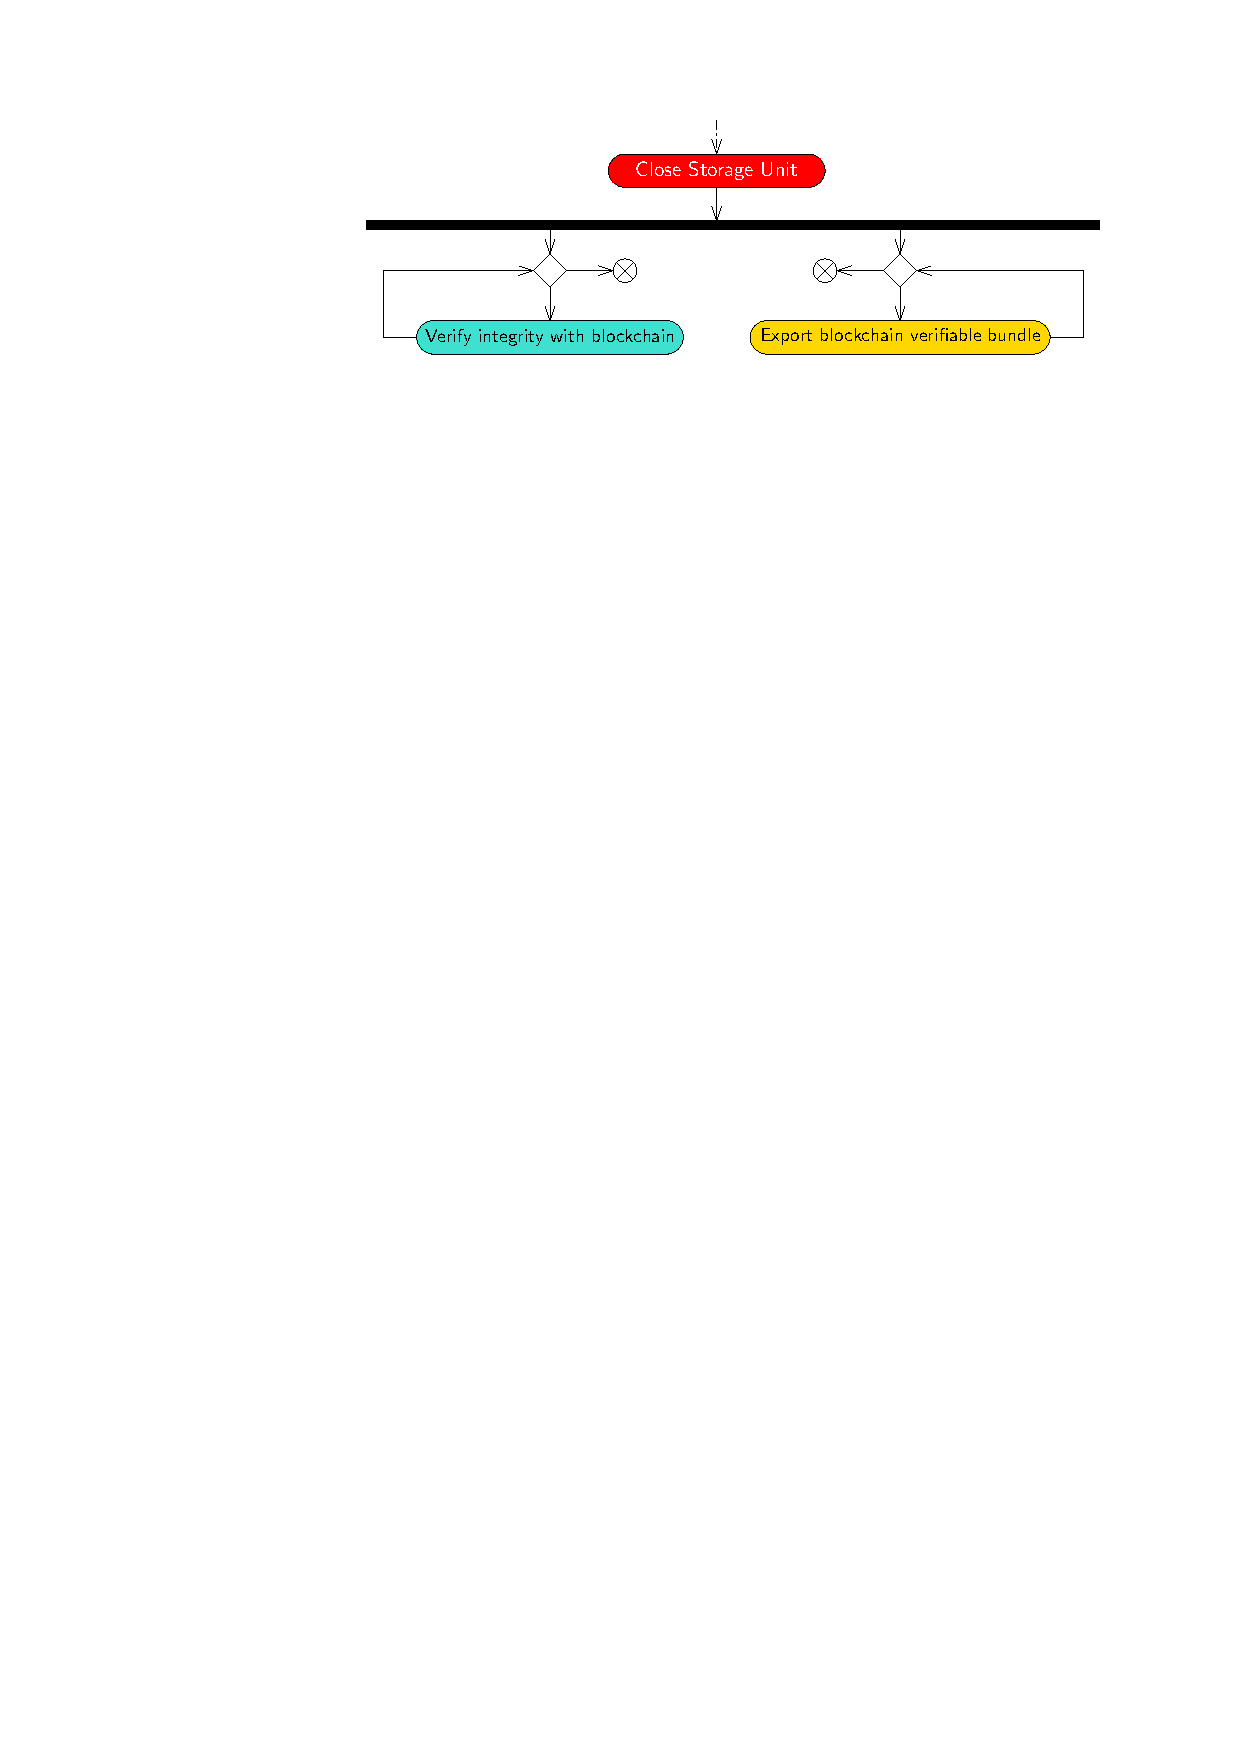
\includegraphics[width=0.8\textwidth]{figures/closed.pdf}
	\end{figure}
	\begin{columns}
		\column{0.4\textwidth}
		\begin{figure}
			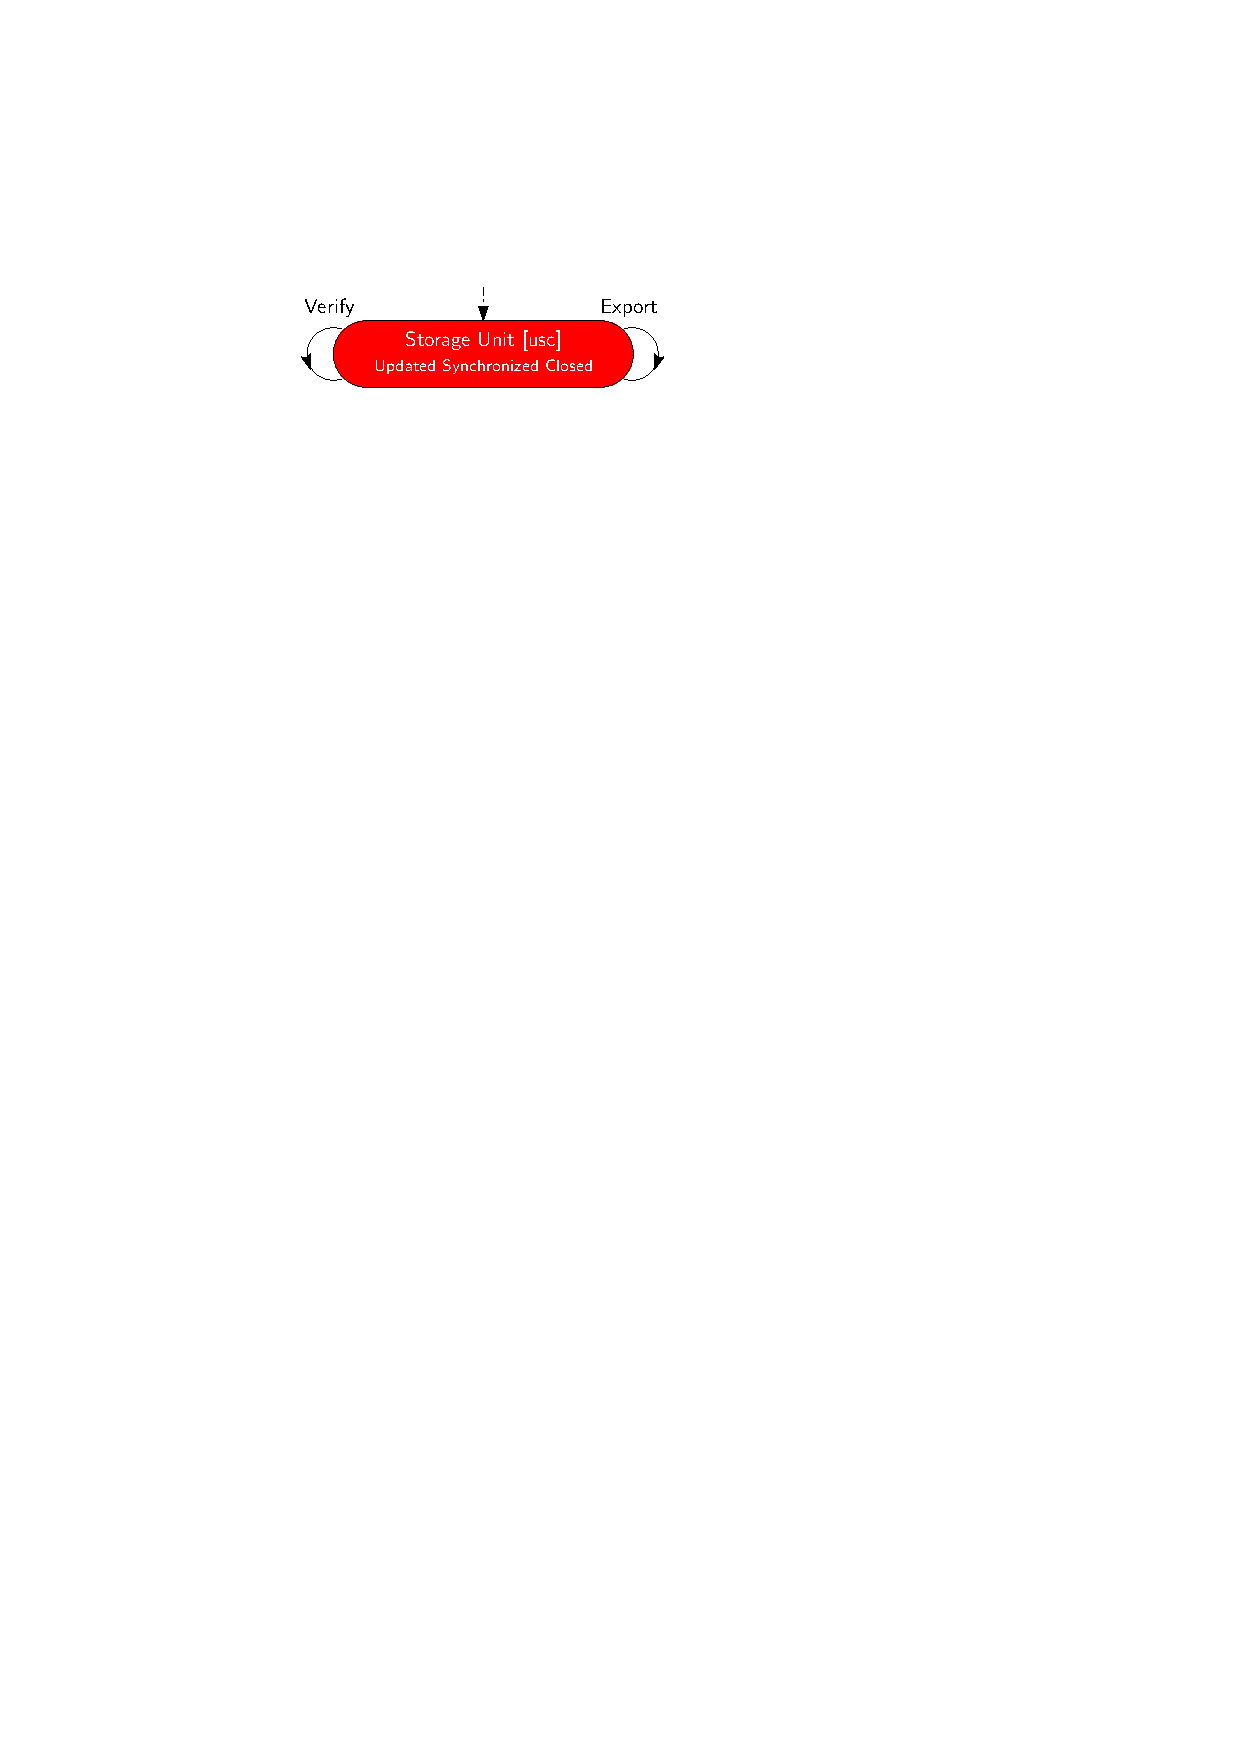
\includegraphics[width=0.8\textwidth]{figures/usc.pdf}
			\bigskip
		\end{figure}
		\column{0.6\textwidth}
		\begin{lstlisting}[language=JavaScript, numbers=none]
			if(fs.existsSync(".pinesu.json")){
				var data = 
				 fs.readFileSync(".pinesu.json")
				var myObj = JSON.parse(data);
				myObj.closed = true;
				fs.writeFileSync(".pinesu.json",
					JSON.stringify(myObj));
				return myObj;
			}
		\end{lstlisting}
	\end{columns}
\end{frame}

\begin{frame}[fragile]
	\frametitle{Esportazione di sottoinsiemi di Storage Unit}
	\begin{figure}
		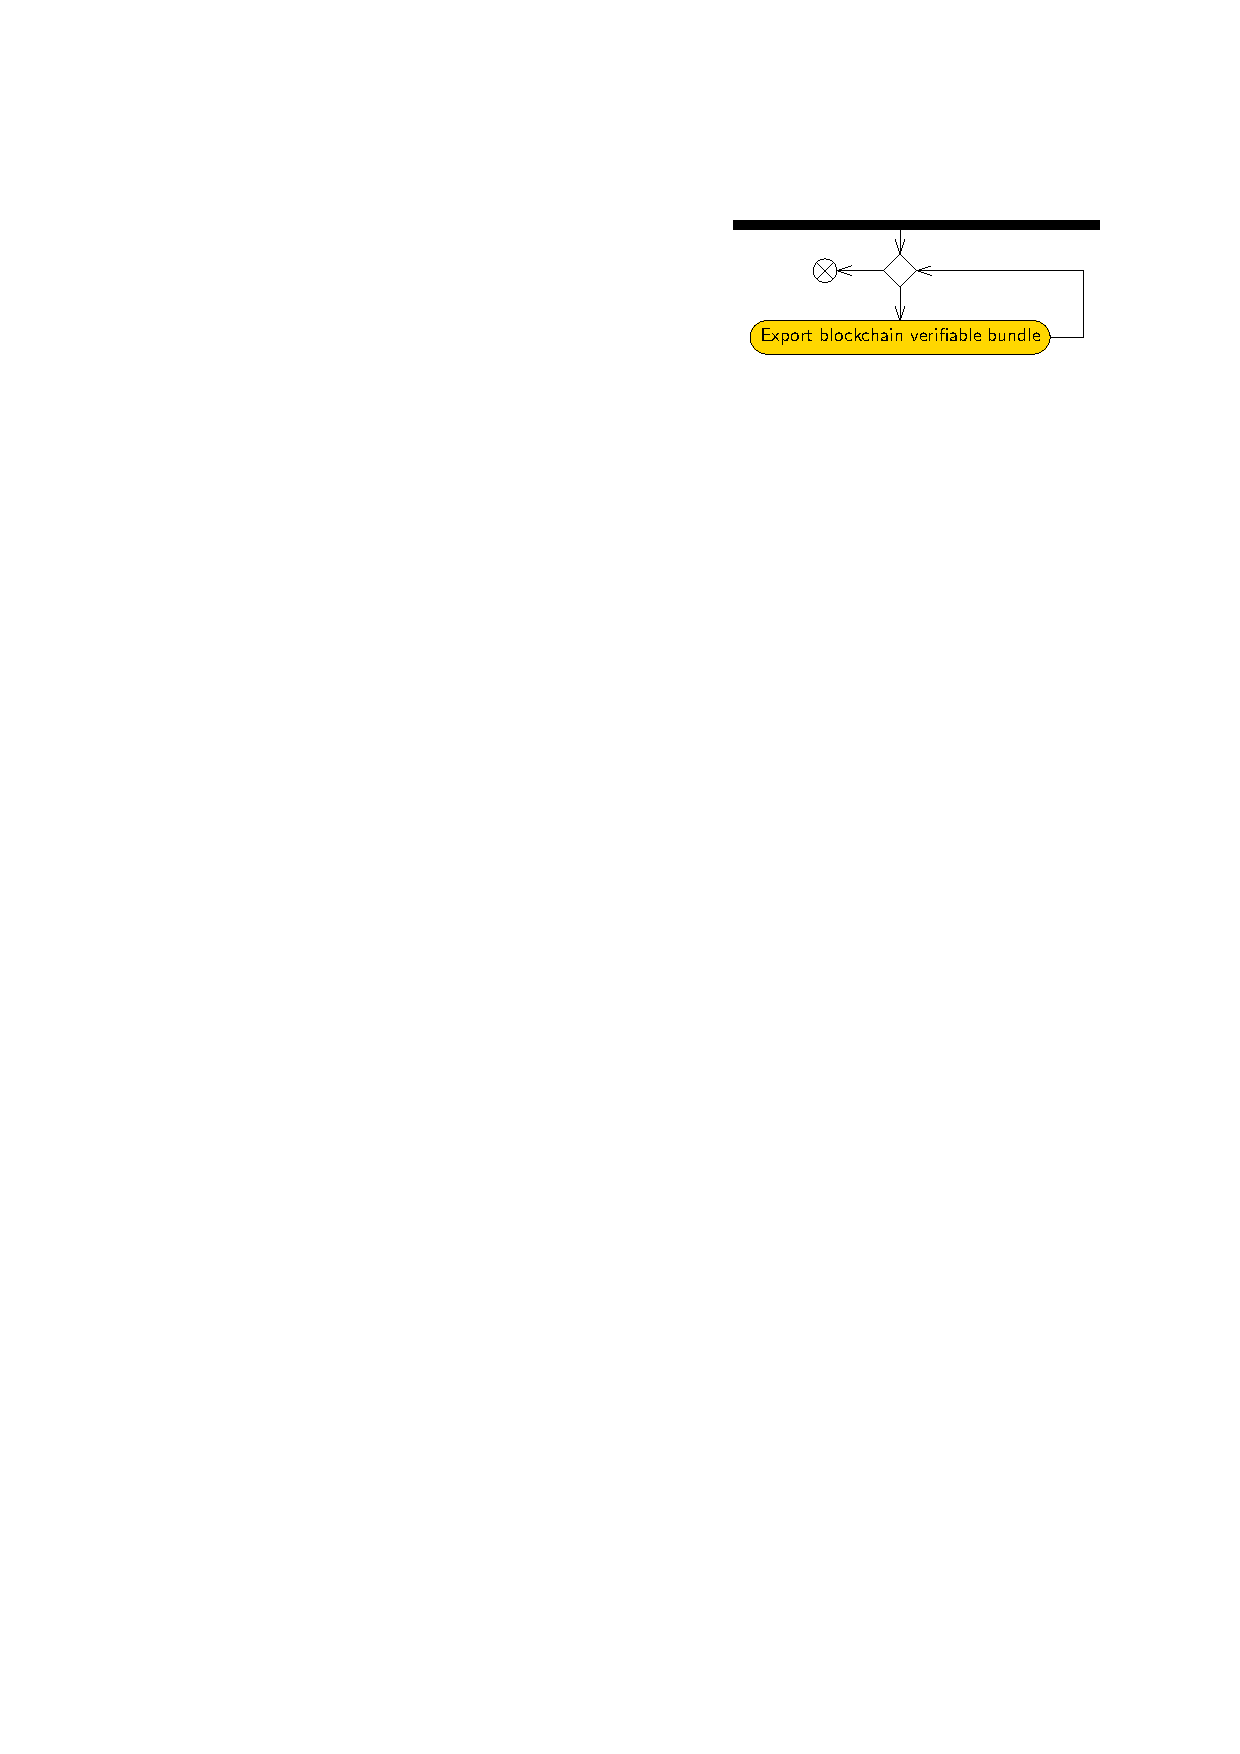
\includegraphics[width=0.6\textwidth]{figures/export.pdf}
	\end{figure}
	\begin{lstlisting}[language=JavaScript, numbers=none]
	var zip = new AdmZip()
	var fl = JSON.stringify(json)
	zip.addFile(".pifiles.json", Buffer.alloc(fl.length, fl))
	for(var el of list){
		zip.addLocalFile(path)
	}
	zip.writeZip("/../pinesuExport.zip")
	\end{lstlisting}
\end{frame}

\begin{frame}[fragile]
	\frametitle{Controllo d'integrità su una Storage Unit}
	\begin{figure}
		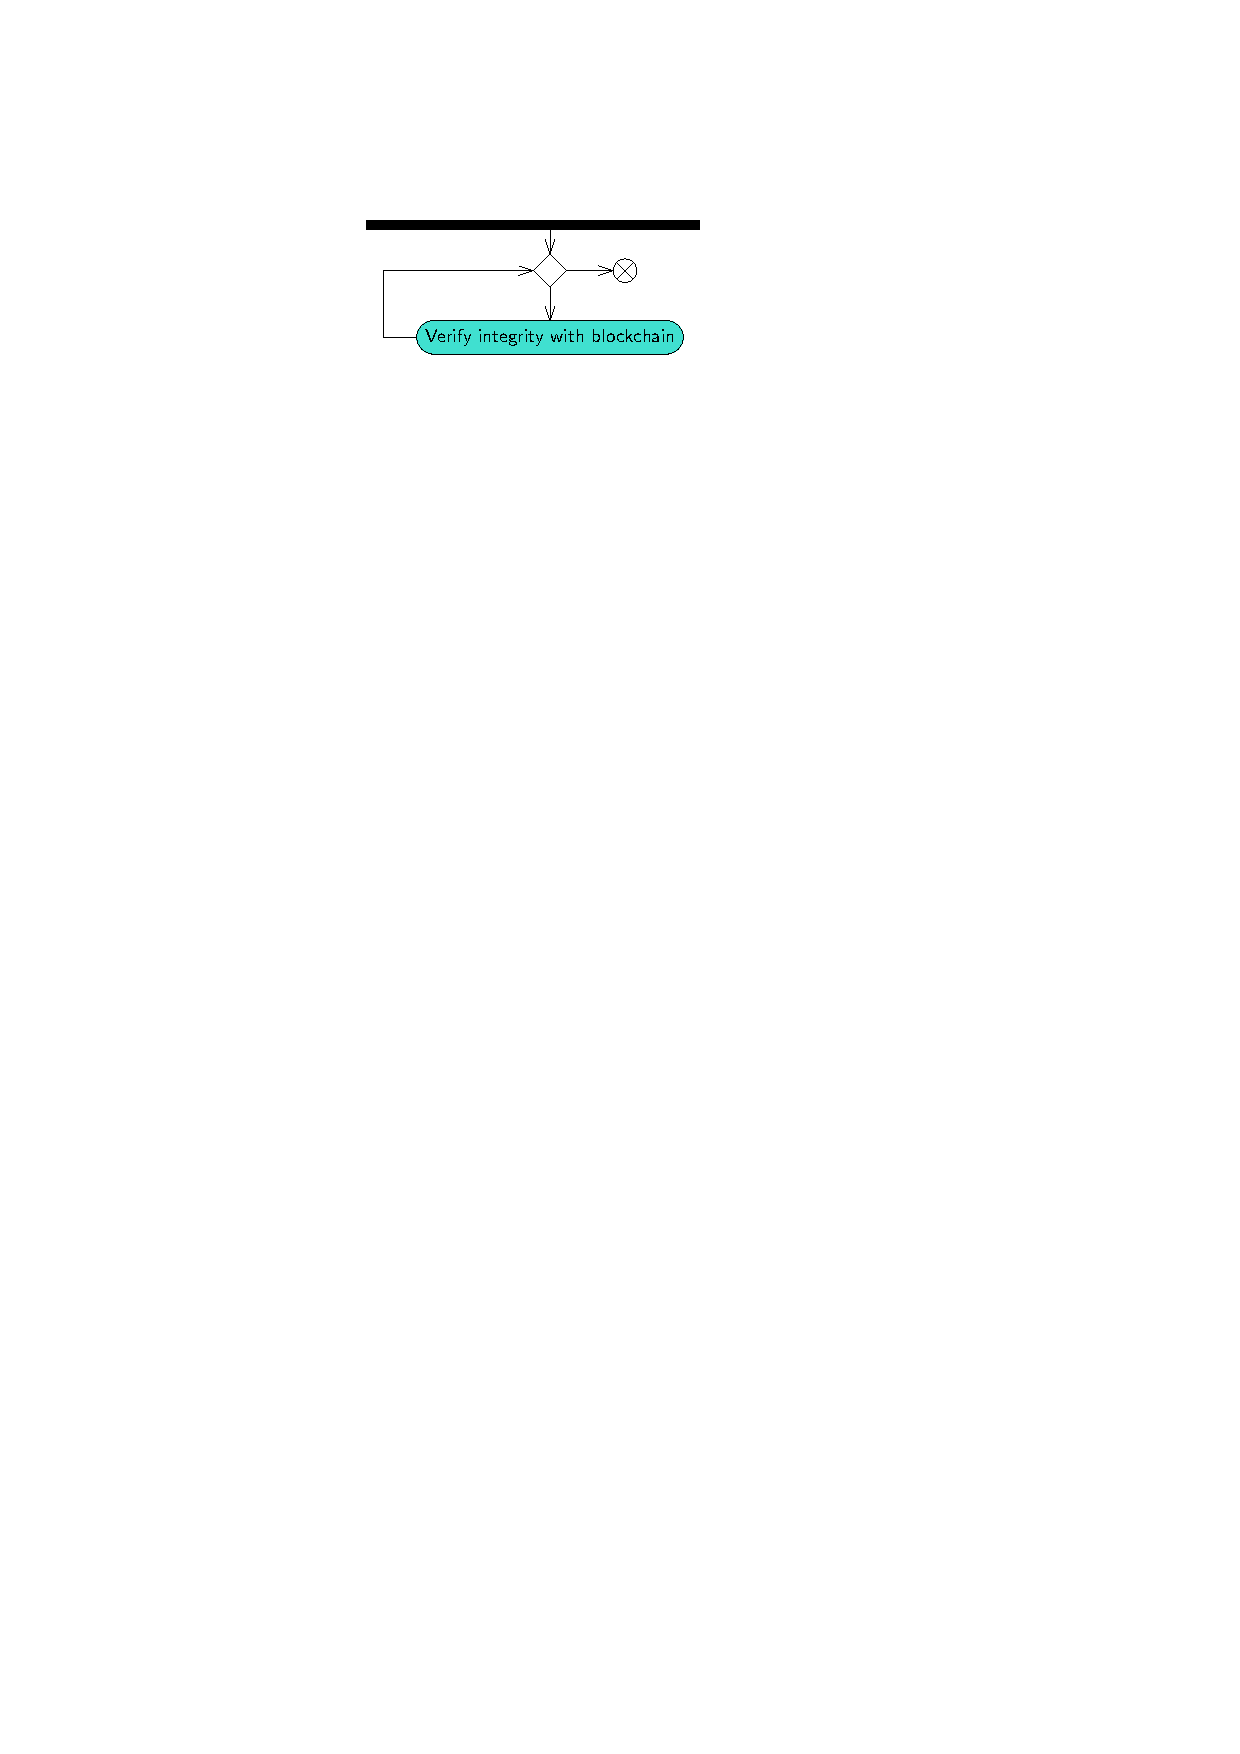
\includegraphics[width=0.6\textwidth]{figures/verify.pdf}
	\end{figure}
	\begin{lstlisting}[language=JavaScript, numbers=none]
	async verifyHash(transHash, hash){
		const res =
			await this.web3.eth.getTransaction(transHash)
		if(res.input == "0x"+hash){
			return true;
		} else {
			return false;
		}
	}
	\end{lstlisting}
\end{frame}

\section{Tecnologie utilizzate}
\begin{frame}
	\frametitle{Node.js}
	\begin{columns}
		\column{0.7\textwidth}
		\textbf{Node.js} è un \textbf{ambiente di run-time},
		che permette di eseguire codice \textbf{Javascript}.
		\smallskip \\
		Esso ha come obiettivi chiave l'\textbf{efficienza} 
		e la \textbf{scalabilità}, può infatti eseguire
		velocemente codice Javascript sia \textbf{server-side}
		che \textbf{client-side}.\\
		\smallskip
		Parte fondamentale di Node sono
		i suoi numerosi \textbf{moduli}: librerie e framework
		realizzati dalla comunità e installabili con facilità
		tramite il package manager \textbf{npm}
		\column{0.3\textwidth}
		\centering
		\begin{figure}
			
\includegraphics[width=\textwidth]{figures/node.png}
		\end{figure} 
	\end{columns}
\end{frame}

\begin{frame}
	\frametitle{Moduli dei connettori}
	\begin{columns}
		\column{0.7\textwidth}
		\textbf{web3.js} è un \textbf{modulo npm} che permette di
		interagire con \textbf{nodi Ethereum} locali e remoti.\\
		\smallskip
		\emph{PineSU EC} lo utilizza per effettuare le transazioni con i
		suoi wallet e per comunicare con lo Smart Contract. \\
		\column{0.3\textwidth}
		\centering
		\begin{figure}
			
\includegraphics[width=\textwidth]{figures/web3.jpg}
		\end{figure} 
	\end{columns}
	\medskip
	\begin{columns}
		\column{0.3\textwidth}
		\centering
		\begin{figure}
			
\includegraphics[width=0.75\textwidth]{figures/gitfw.png}
		\end{figure} 
		\column{0.7\textwidth}
		\textbf{Simple Git} è un \textbf{modulo npm} che permette di
		comunicare con il client Git locale. \\
		\smallskip
		Usato in \emph{PineSU GC}, esso permette l'esecuzione di
		comandi in maniera \textbf{asincrona}. \\
	\end{columns}
\end{frame}

\begin{frame}
	\frametitle{Altri moduli}
	\begin{columns}
		\column{0.3\textwidth}
		\centering
		\begin{figure}
			
\includegraphics[width=0.75\textwidth]{figures/inquirer.png}
		\end{figure} 
		\column{0.7\textwidth}
		\textbf{Inquirer.js} è un \textbf{modulo npm} che facilita
		la creazione di \textbf{interfacce utente} tramite menù testuali. \\
		\smallskip
		In \emph{PineSU CLI} viene usato per \textbf{interagire}
		con l'utente ponendogli \textbf{domande} dalla risposta chiusa o aperta. \\
	\end{columns}
	\medskip
	\begin{columns}
		\column{0.7\textwidth}
		\textbf{ADM-ZIP} è un \textbf{modulo npm} che consente di
		creare cartelle compresse in formato ZIP.\\
		\smallskip
		\emph{PineSU BEL} lo utilizza per \textbf{esportare sottoinsiemi} di
		SU mantenendo la \textbf{struttura gerarchica} originale. \\
		\column{0.3\textwidth}
		\centering
		\begin{figure}
			
\includegraphics[width=\textwidth]{figures/zip.png}
		\end{figure} 
	\end{columns}
\end{frame}

\section{Sviluppi futuri}
\begin{frame}
	\frametitle{Sviluppi futuri}
	\begin{enumerate}
		\item Migliorare gestione degli \textbf{accumulatori crittografici} per le \textbf{singole SU}.
		\item Implementare \textbf{Smart Contract} dalle migliori funzionalità.
		\item Aggiungere \textbf{connettori} per \textbf{ulteriori blockchain}.
		\item Creare \textbf{portale web} con \textbf{server Git} per la gestione remota delle SU (\emph{ambizioso}).
	\end{enumerate}
\end{frame}

%\section{Fonti}
%\begin{frame}
%	\frametitle{Fonti}
%	\begin{itemize}
%		\item \href{https://ethereum.org/it/developers/}{Strumenti Ethereum per sviluppatori} 
%  		\item \href{https://www.trufflesuite.com/tutorial}{Tutorial Truffle DAPPs - Pet Shop}
%  		\item \href{https://www.sitepoint.com/javascript-command-line-interface-cli-node-js/}{Build a JavaScript CLI with Node.js}
%  		\item \href{https://developer.mozilla.org/en-US/docs/Learn/JavaScript/Asynchronous/Async_await}{Tutorial di Mozilla su async / await}
%  		\item Immagini reperite dai siti ufficiali degli strumenti eccetto per alcune scaricate da queste pagine web:
%			\begin{itemize}
%				\item \href{https://www.poeticoding.com/hashing-a-file-in-elixir/}{Funzioni di Hashing}
%				\item \href{https://www.romatoday.it/attualita/concorso-rai-fiera-roma-norme-covid-19.html}{Concorso pubblico}
%				\item \href{https://www.criptovalute24.com/ethereum-migliora-la-sua-blockchain-rialzo-del-5-4/}{Ethereum Blockchain}
%				\item \href{https://blog.netsons.com/git-software-guida-facile/}{Git repository}
%				\item \href{https://amerlin.keantex.com/programmazione-asincrona-con-async-await-parte-2/}{async / await}
%				\item \href{https://transparency.dev/verifiable-data-structures/}{Merkle Tree}
%			\end{itemize}
%			\item \href{https://waifu2x.booru.pics/Home/index}{Strumento di upscaling delle immagini} 
%	\end{itemize}
%\end{frame}

\end{document}